\documentclass[aspectratio=169]{beamer}

\usetheme{default}
\usefonttheme{professionalfonts}
\setbeamertemplate{navigation symbols}{}
\setbeamertemplate{itemize items}[circle]
\setbeamercolor{itemize item}{fg=white}

\setbeamerfont{title}{series=\bfseries, size=\normalfont\Large}
\setbeamercolor{title}{fg=white}

\setbeamerfont{author}{size=\normalfont\small}
\setbeamercolor{author}{fg=white}

\setbeamerfont{frametitle}{series=\bfseries, size=\normalfont}
\setbeamercolor{frametitle}{fg=white}

\setbeamerfont{framesubtitle}{size=\normalfont\large}
\setbeamercolor{framesubtitle}{fg=white}

\setbeamercolor{background canvas}{bg=black}
\setbeamercolor{normal text}{fg=white}

\usepackage[utf8]{inputenc}
\usepackage[french]{babel}
\usepackage{amsmath}
\usepackage{amsfonts}
\usepackage{amssymb}
\usepackage{graphicx}
\usepackage[]{bm}
\usepackage[]{multimedia}
\usepackage[]{multicol}
\usepackage[squaren,Gray]{SIunits}

\graphicspath{{imgs/}}

\usepackage{tikz} % Required for drawing custom shapes
\usetikzlibrary{arrows}
\usetikzlibrary{shapes.geometric, math, positioning, calc, patterns, angles, quotes}
\usetikzlibrary{patterns.meta,decorations.pathmorphing}




\usepackage[]{listings}

\definecolor{codegreen}{rgb}{0,0.8,0}
\definecolor{codegray}{rgb}{0.5,0.5,0.5}
%\definecolor{codepurple}{rgb}{0.58,0,0.82}
\definecolor{codepurple}{rgb}{0,0.8,0}
\definecolor{backcolour}{rgb}{0.0, 0.0, 0.0}

\lstdefinestyle{mystyle}{
  backgroundcolor=\color{backcolour},
  commentstyle=\color{codegreen},
  keywordstyle=\color{magenta},
  numberstyle=\tiny\color{codegray},
  stringstyle=\color{codepurple},
  basicstyle=\ttfamily\footnotesize,
  breakatwhitespace=false,
  breaklines=true,
  captionpos=b,
  keepspaces=true,
  numbers=left,
  numbersep=5pt,
  showspaces=false,
  showstringspaces=false,
  showtabs=false,
  tabsize=2
}

\lstset{style=mystyle}



\title{Introduction à Python}
\author{Jean-Christophe LOISEAU}
\institute{Arts \& Métiers Institute of Technology, 2021-2022}
\date{}

\begin{document}





\frame{\titlepage}





\begin{frame}[fragile]{}{}
  \begin{minipage}{.64\textwidth}
    \textbf{\alert{Matplotlib}} : Package \verb+Python+ pour tracer et visualiser des données sous forme de graphiques ou d'animations.
  \end{minipage}%
  \hfill
  \begin{minipage}{.32\textwidth}
    \centering
    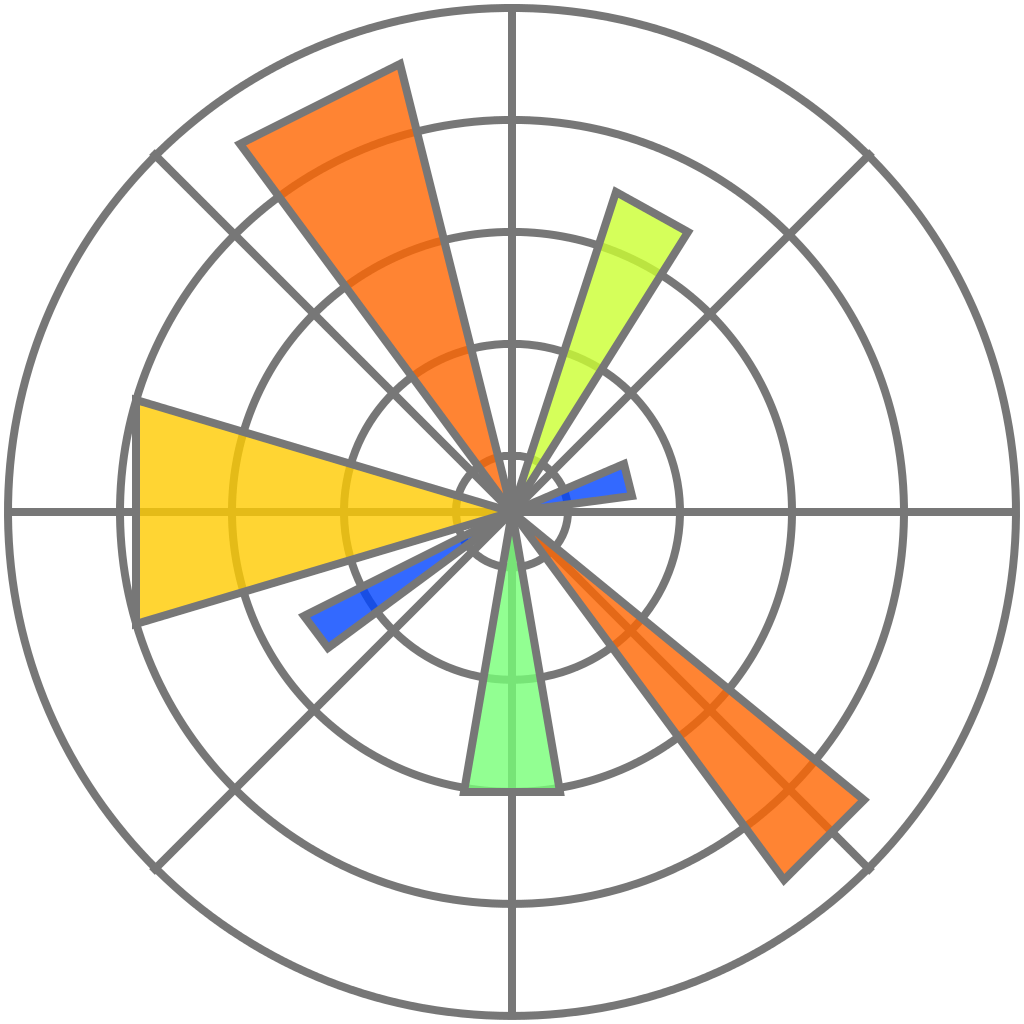
\includegraphics[width=.75\textwidth]{matplotlib_logo}
  \end{minipage}

  \vspace{-1cm}
\end{frame}





\frame{}




\begin{frame}[fragile]{}{}
  \vfill
  \begin{lstlisting}[language=Python]
    import numpy as np
    import matplotlib.pyplot as plt
  \end{lstlisting}
  \vfill
\end{frame}





\begin{frame}
  \vfill
  \centering
  \textbf{Tracer des courbes}
  \vfill
\end{frame}

{
  \setbeamercolor{background canvas}{bg=white}
  \frame{
    \vfill
    \centering
    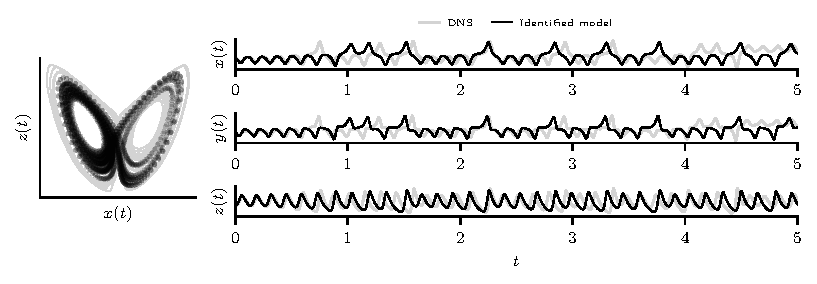
\includegraphics[width=\textwidth]{attractor_comparison_bis}
    \vfill
  }
}




\begin{frame}[fragile]{}{}
  \vfill
  \begin{minipage}{.48\textwidth}
    \begin{lstlisting}[language=Python]
      # Donnees synthetiques.
      x = np.linspace(-6, 6, 128)
      y = np.cos(x)

      # Cree une figure.
      plt.figure()

      # Plot par defaut.
      plt.plot(x, y)

      # Affiche le graphe
      plt.show()
    \end{lstlisting}
  \end{minipage}%
  \hfill
  \begin{minipage}{.48\textwidth}
    \centering
    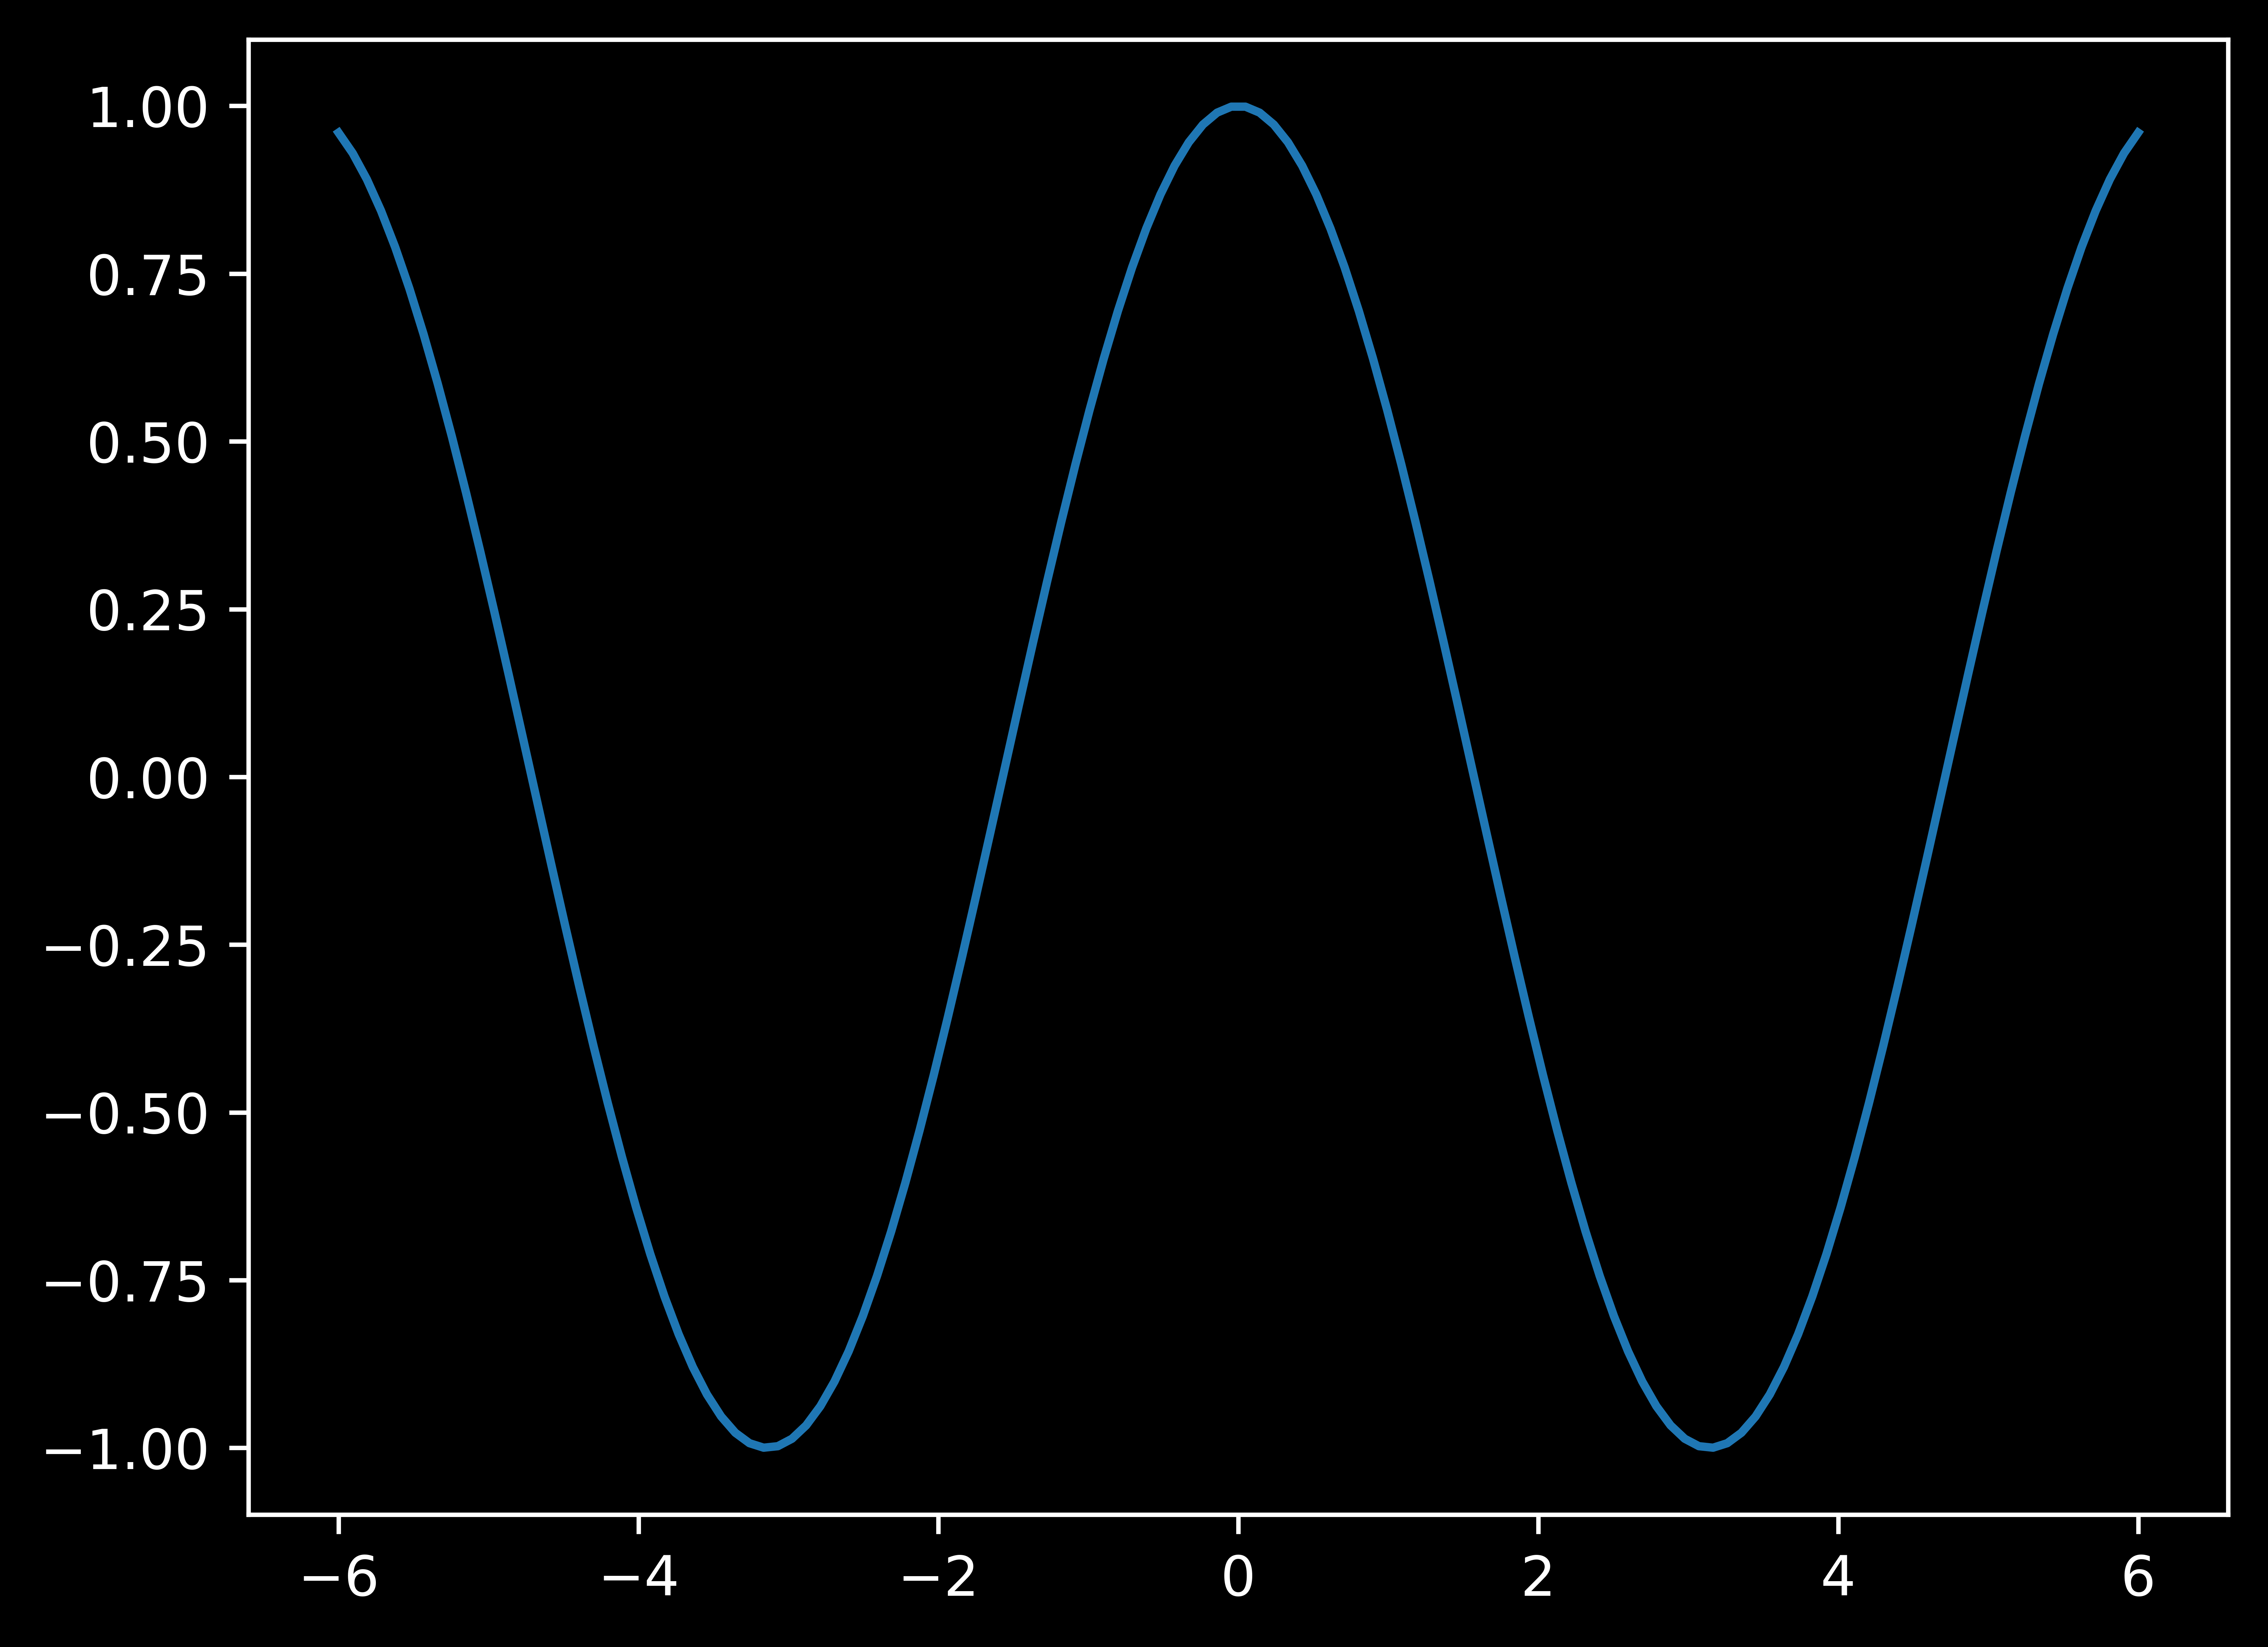
\includegraphics[width=\textwidth]{line_plot_default}
  \end{minipage}
  \vfill
\end{frame}

\begin{frame}[fragile]{}{}
  \vfill
  \begin{minipage}{.48\textwidth}
    \begin{lstlisting}[language=Python]

      # Titres des axes.
      plt.xlabel('x')
      plt.ylabel('y')

      # Titre de la figure.
      plt.title('y = cos(x)')
    \end{lstlisting}
  \end{minipage}%
  \hfill
  \begin{minipage}{.48\textwidth}
    \centering
    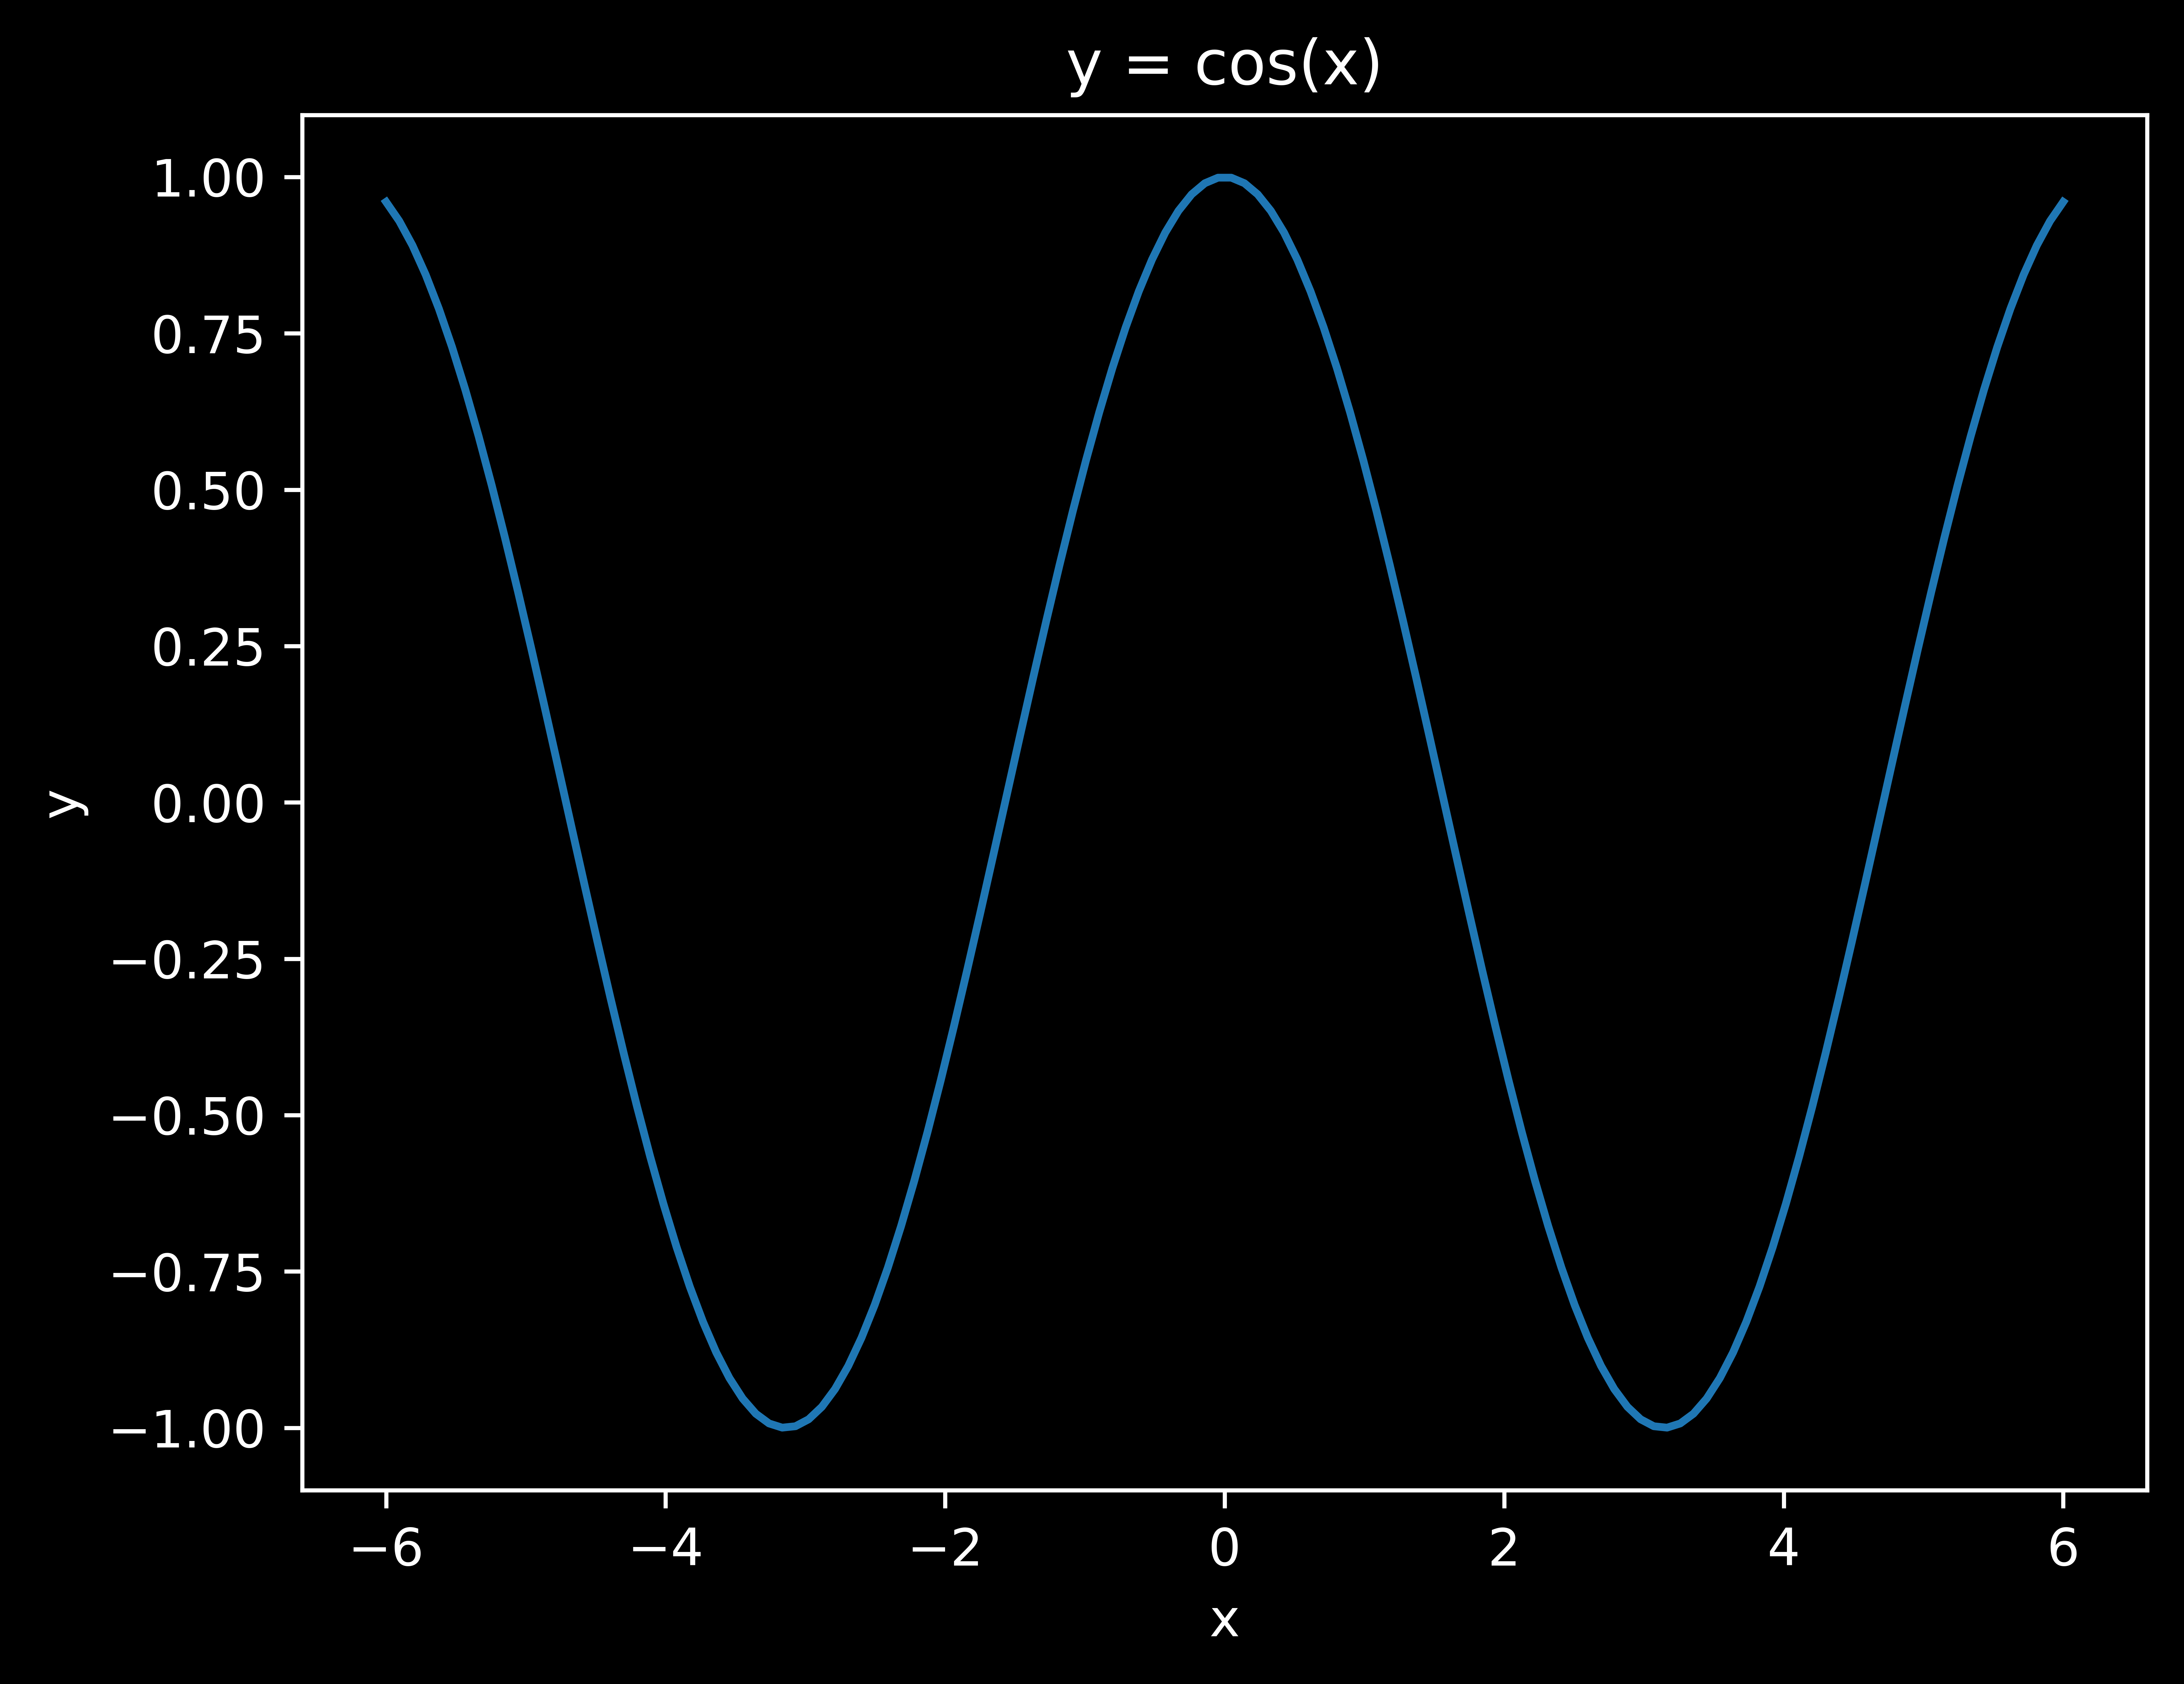
\includegraphics[width=\textwidth]{line_plot_labels}
  \end{minipage}
  \vfill
\end{frame}


\begin{frame}[fragile]{}{}
  \vfill
  \begin{minipage}{.48\textwidth}
    \begin{lstlisting}[language=Python]

      # Limites des axes.
      plt.xlim(-6, 6)
      plt.ylim(-1, 1)
    \end{lstlisting}
  \end{minipage}%
  \hfill
  \begin{minipage}{.48\textwidth}
    \centering
    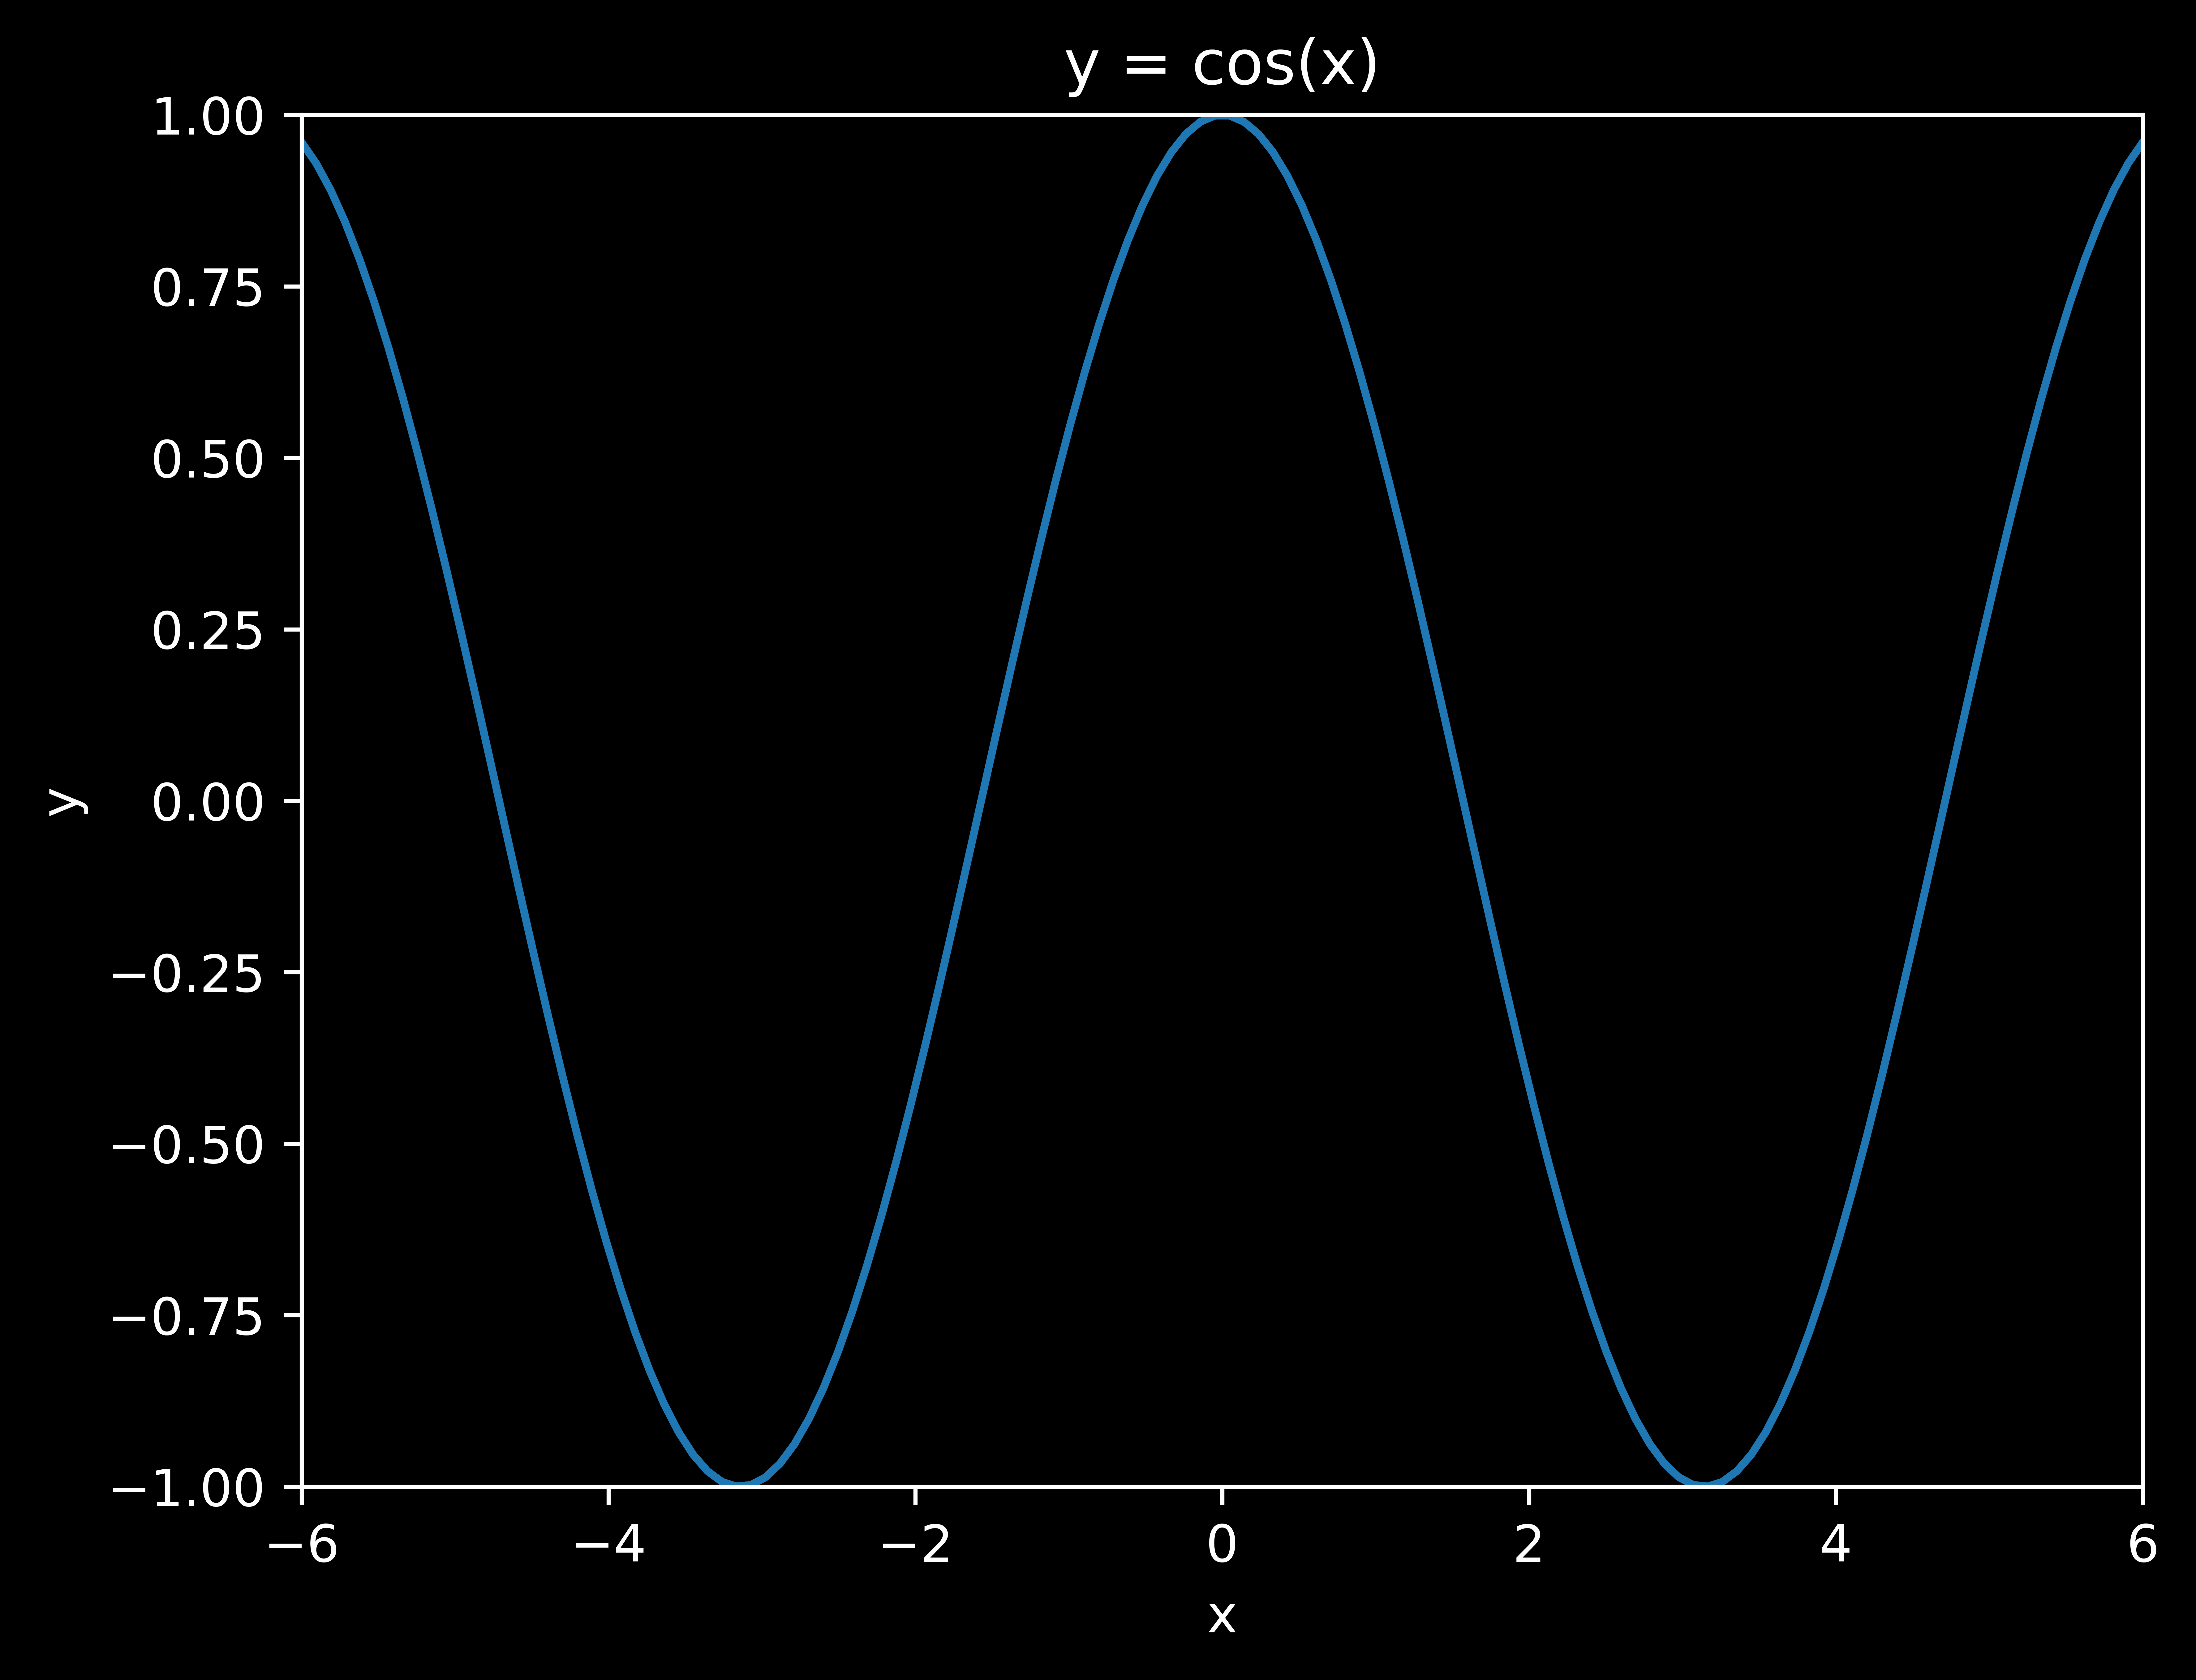
\includegraphics[width=\textwidth]{line_plot_limits}
  \end{minipage}
  \vfill
\end{frame}


\begin{frame}[fragile]{}{}
  \vfill
  \begin{minipage}{.48\textwidth}
    \begin{lstlisting}[language=Python]

      # Proprietes de la courbe.
      plt.plot(x, y, c='r', lw=3)
    \end{lstlisting}
  \end{minipage}%
  \hfill
  \begin{minipage}{.48\textwidth}
    \centering
    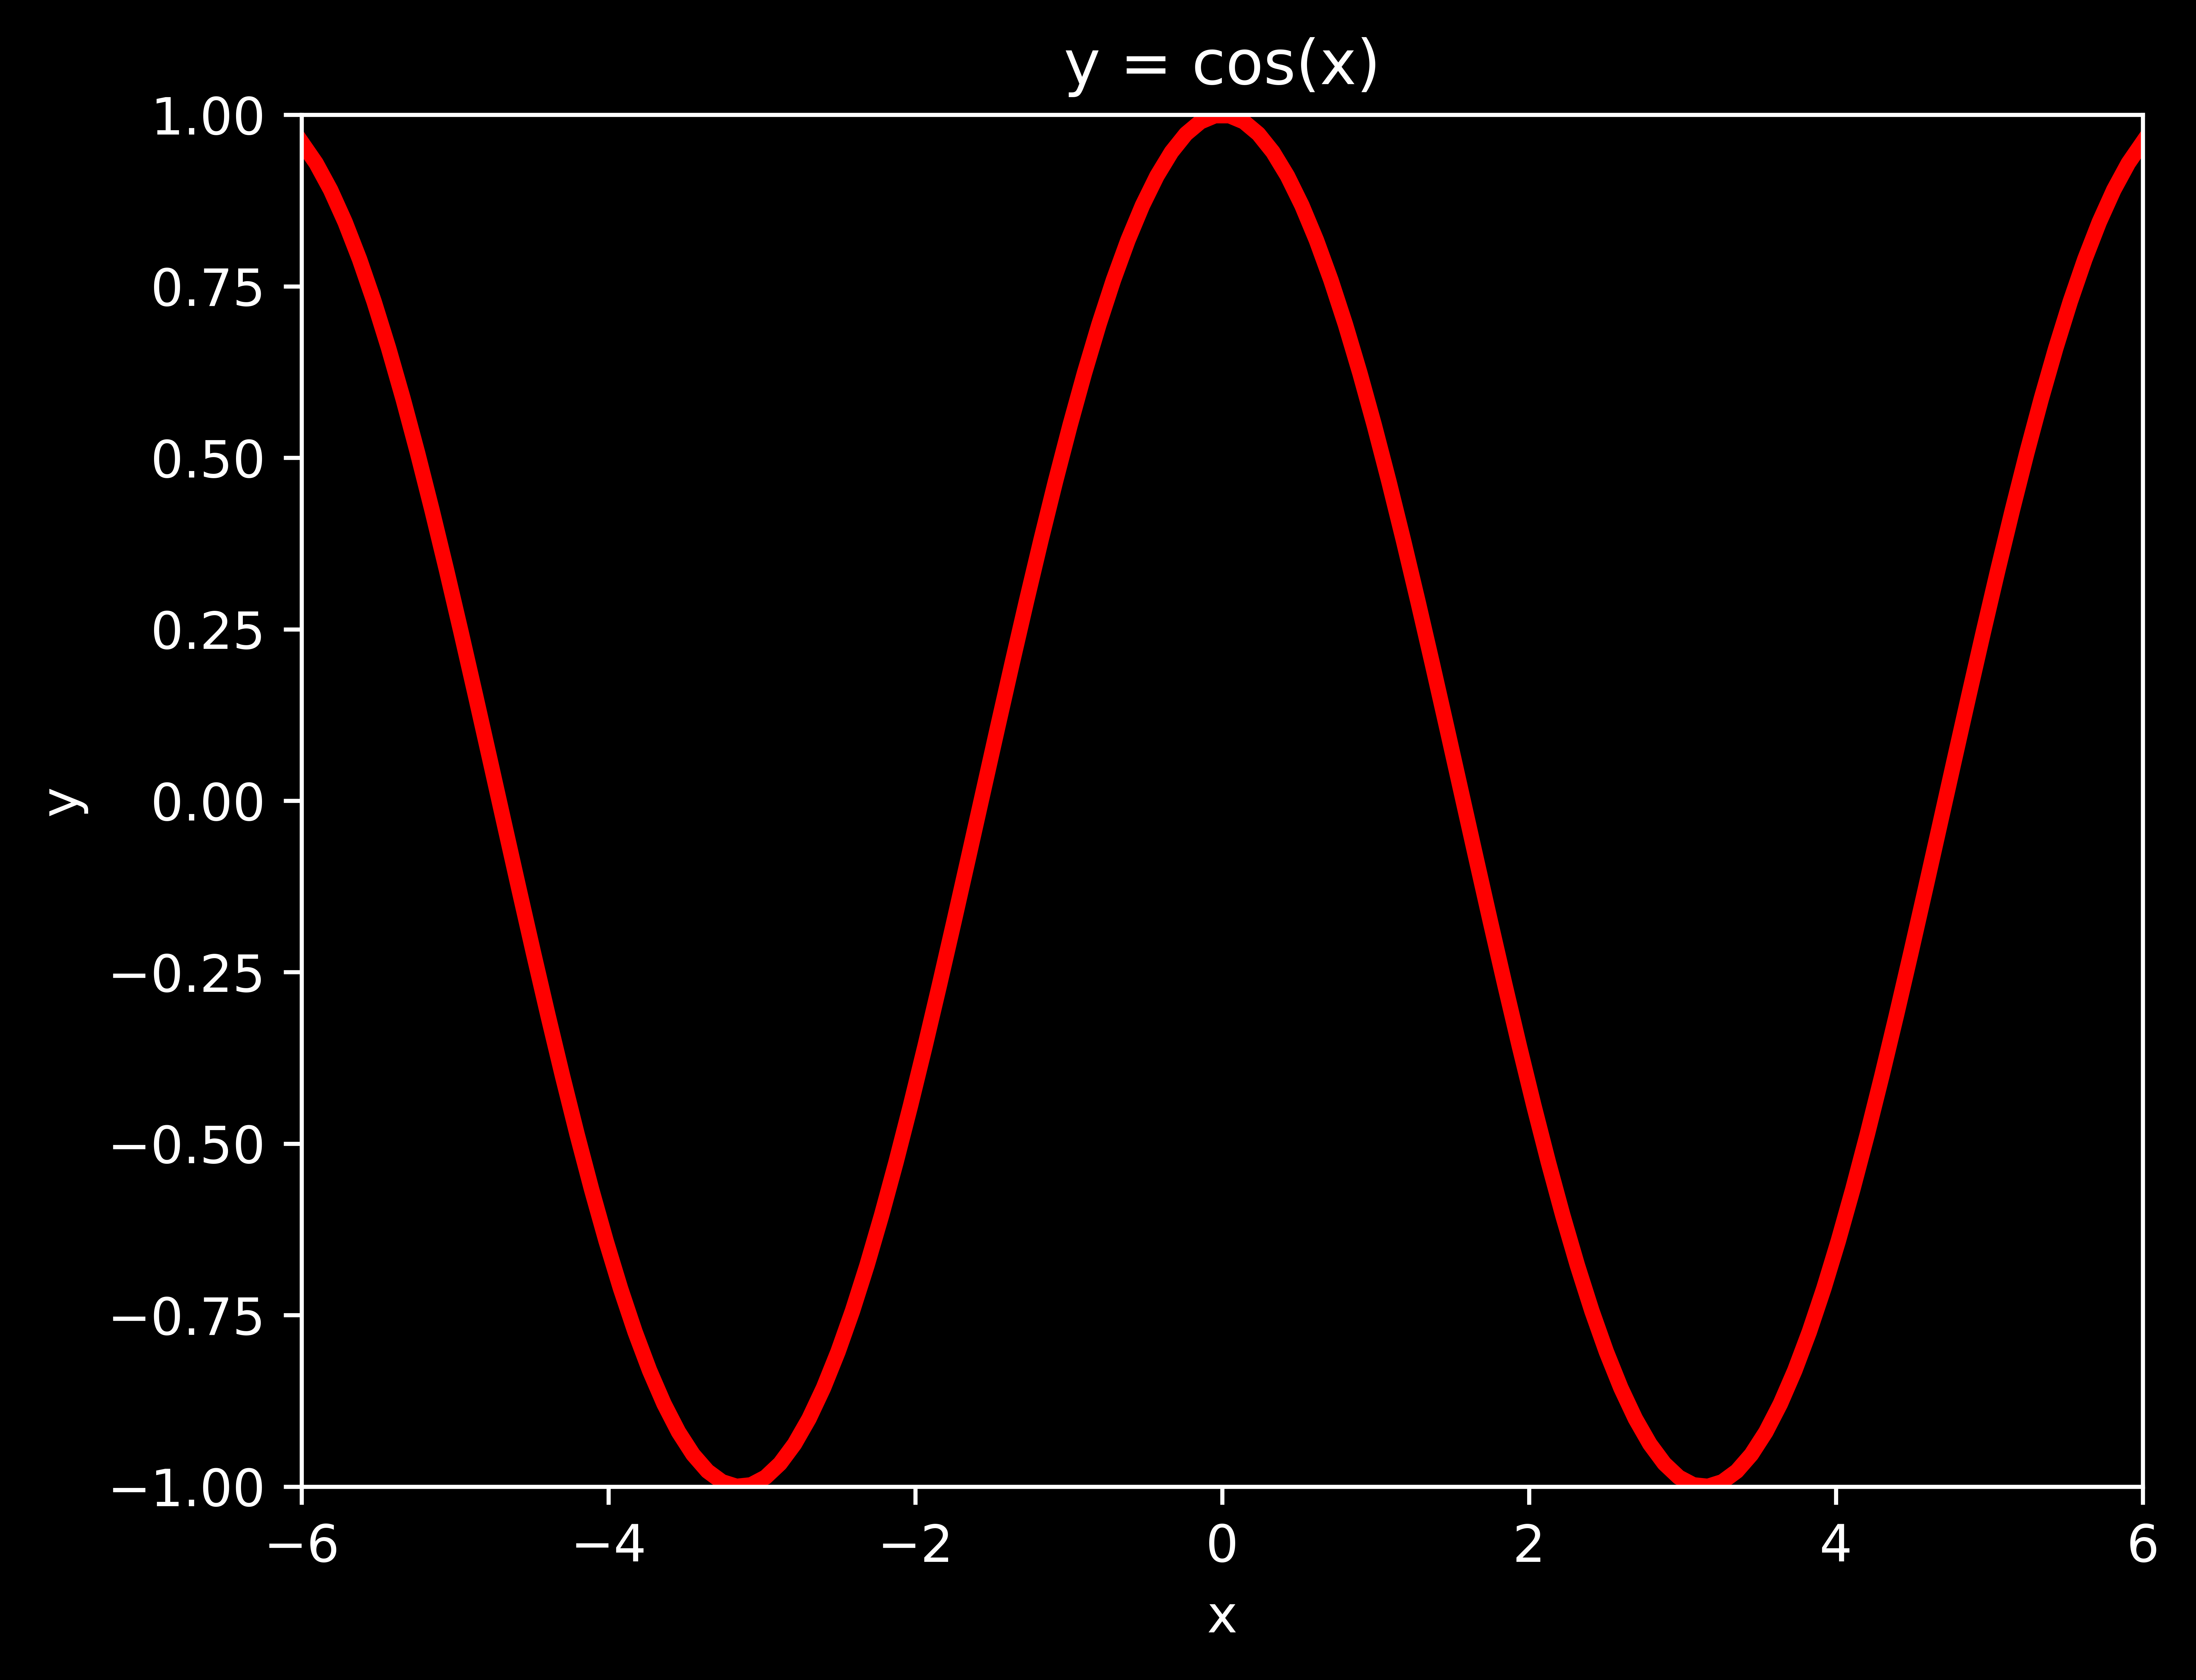
\includegraphics[width=\textwidth]{line_plot_color}
  \end{minipage}
  \vfill
\end{frame}

\frame{}

\begin{frame}[fragile]{}{}
  \vfill
  \begin{minipage}{.48\textwidth}
    \begin{lstlisting}[language=Python]
      # Donnees synthetiques.
      x = np.linspace(-6, 6, 128)
      y = np.cos(x)
      z = np.sin(x)

      # Cree une figure.
      plt.figure()

      # Plot par defaut.
      plt.plot(x, y)
      plt.plot(x, z)

      plt.show()
    \end{lstlisting}
  \end{minipage}%
  \hfill
  \begin{minipage}{.48\textwidth}
    \centering
    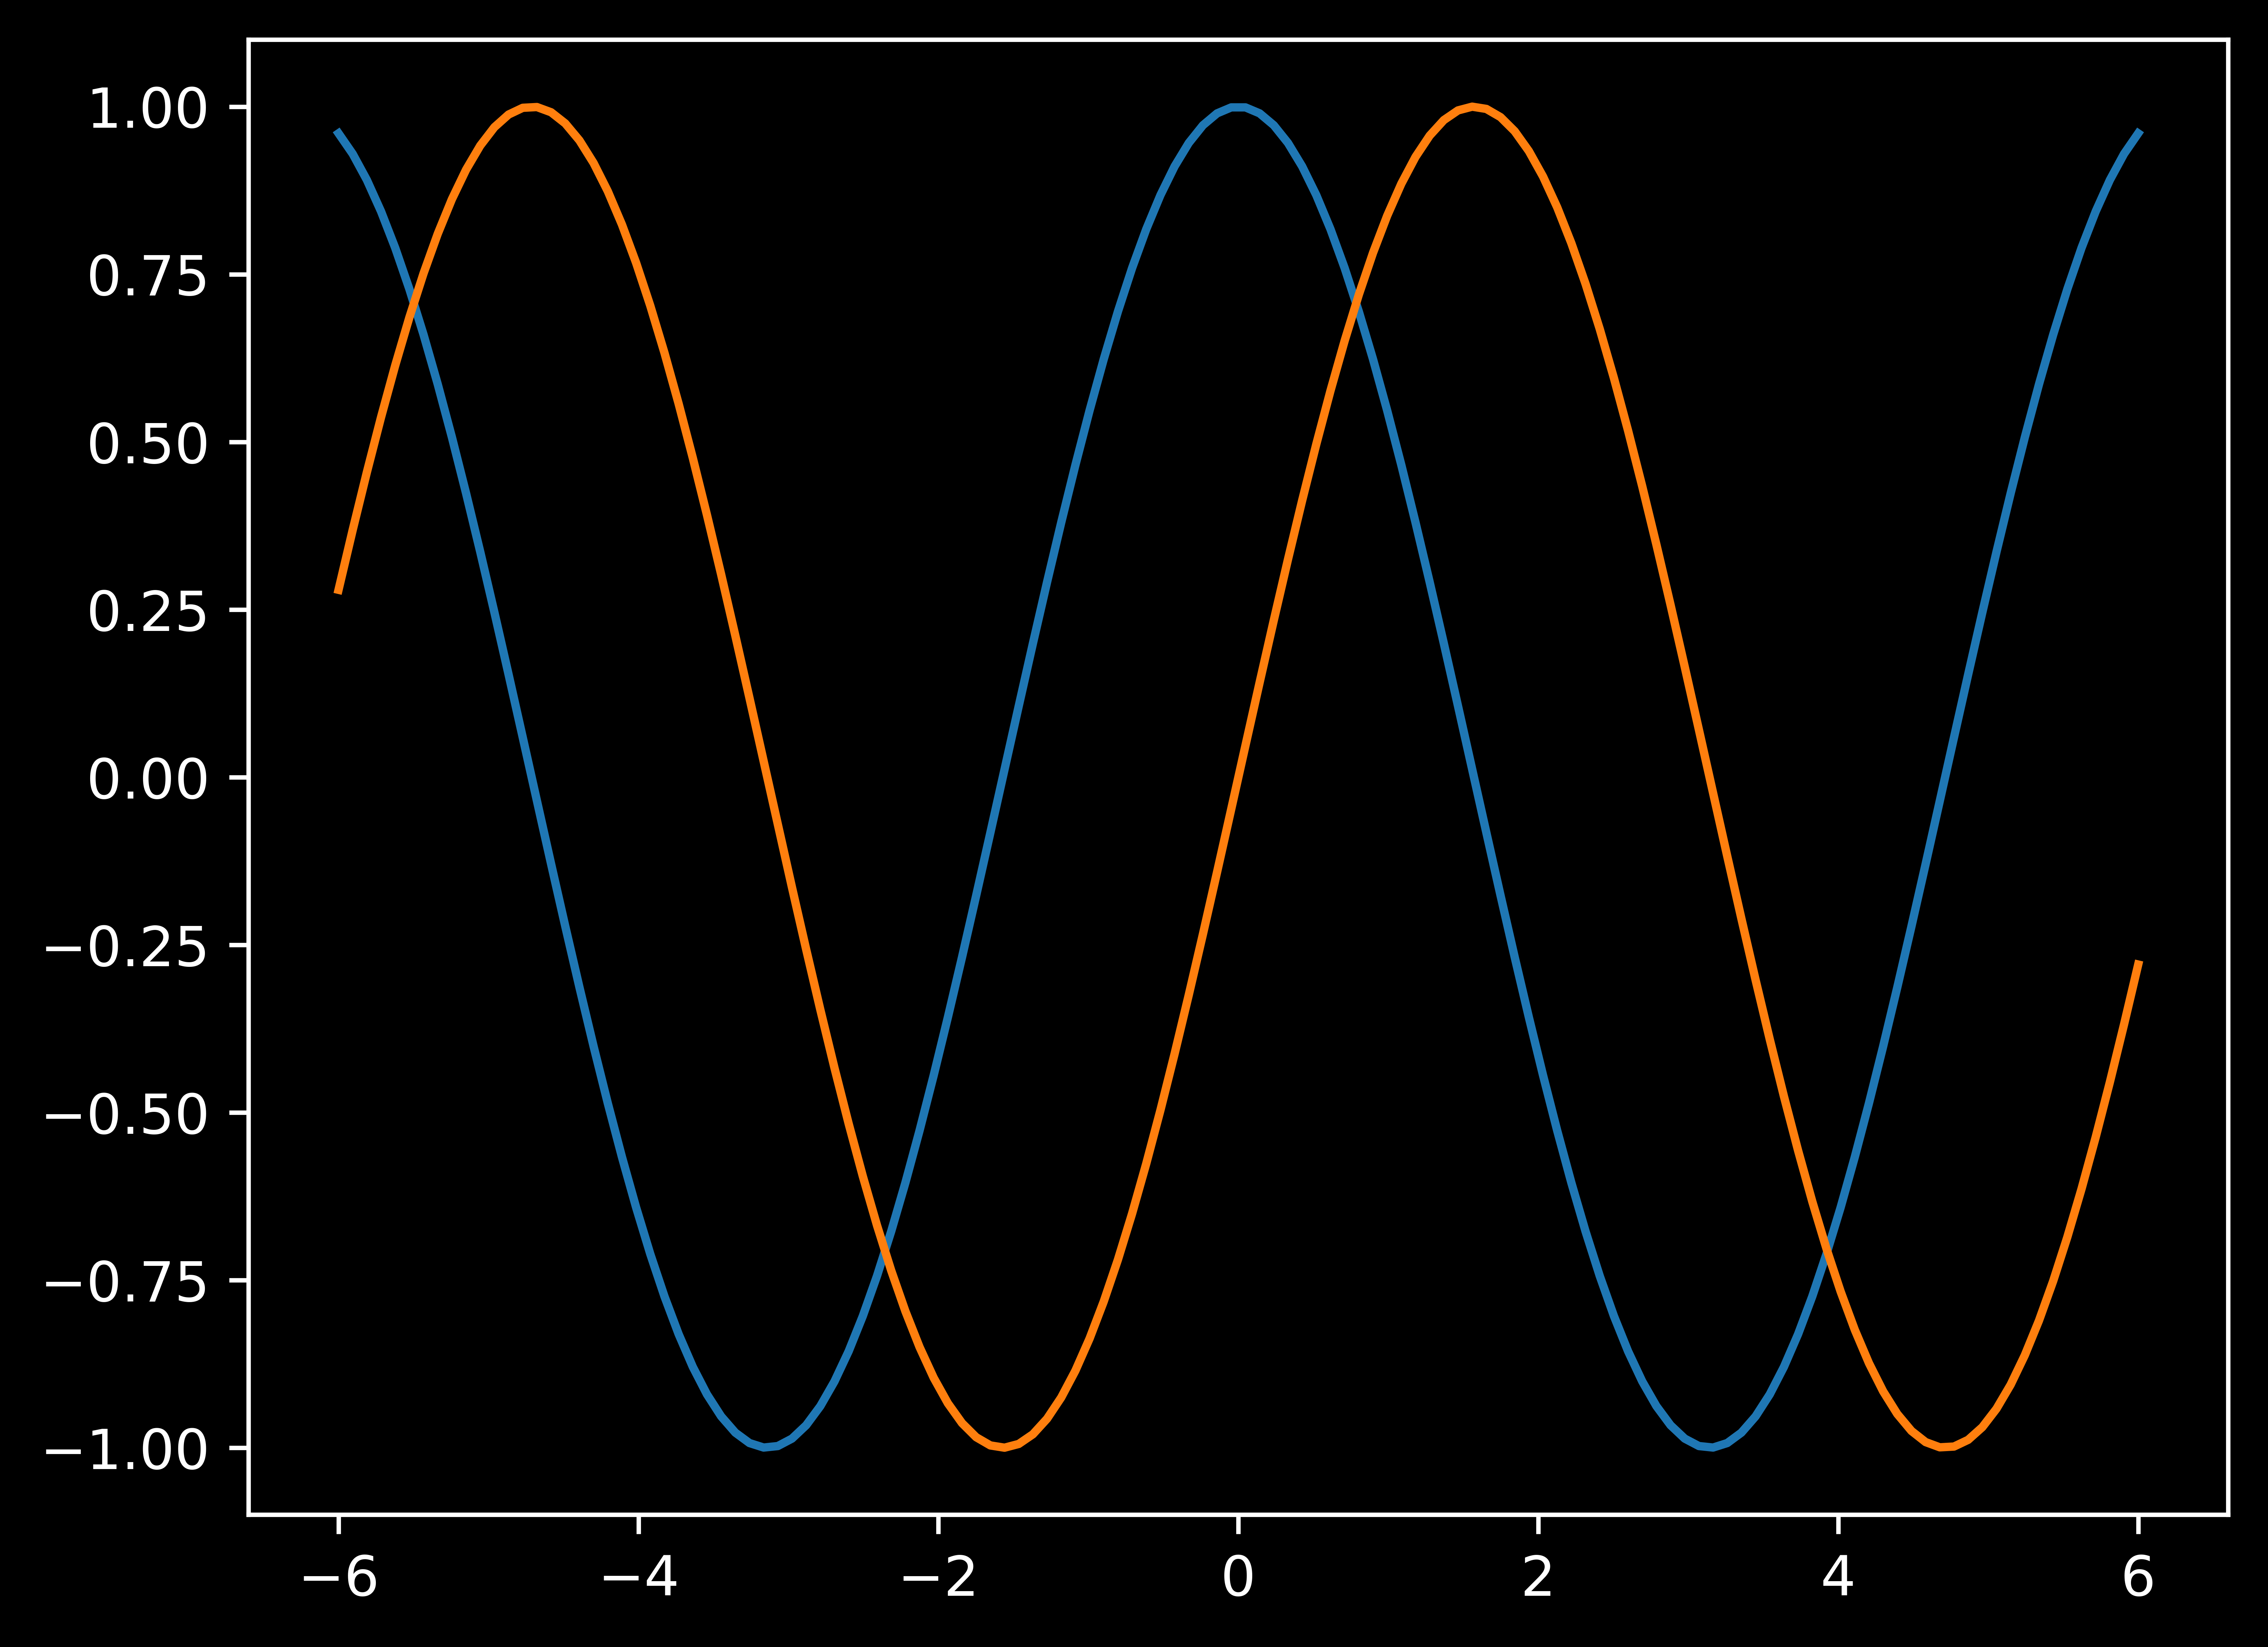
\includegraphics[width=\textwidth]{mline_plot_default}
  \end{minipage}
  \vfill
\end{frame}





\begin{frame}[fragile]{}{}
  \vfill
  \begin{minipage}{.48\textwidth}
    \begin{lstlisting}[language=Python]
      # Noms des courbes.
      plt.plot(
          x, y,
          label='cosinus')
      plt.plot(
          x, z,
          label='sinus')

      # Ajoute la legende.
      plt.legend()
    \end{lstlisting}
  \end{minipage}%
  \hfill
  \begin{minipage}{.48\textwidth}
    \centering
    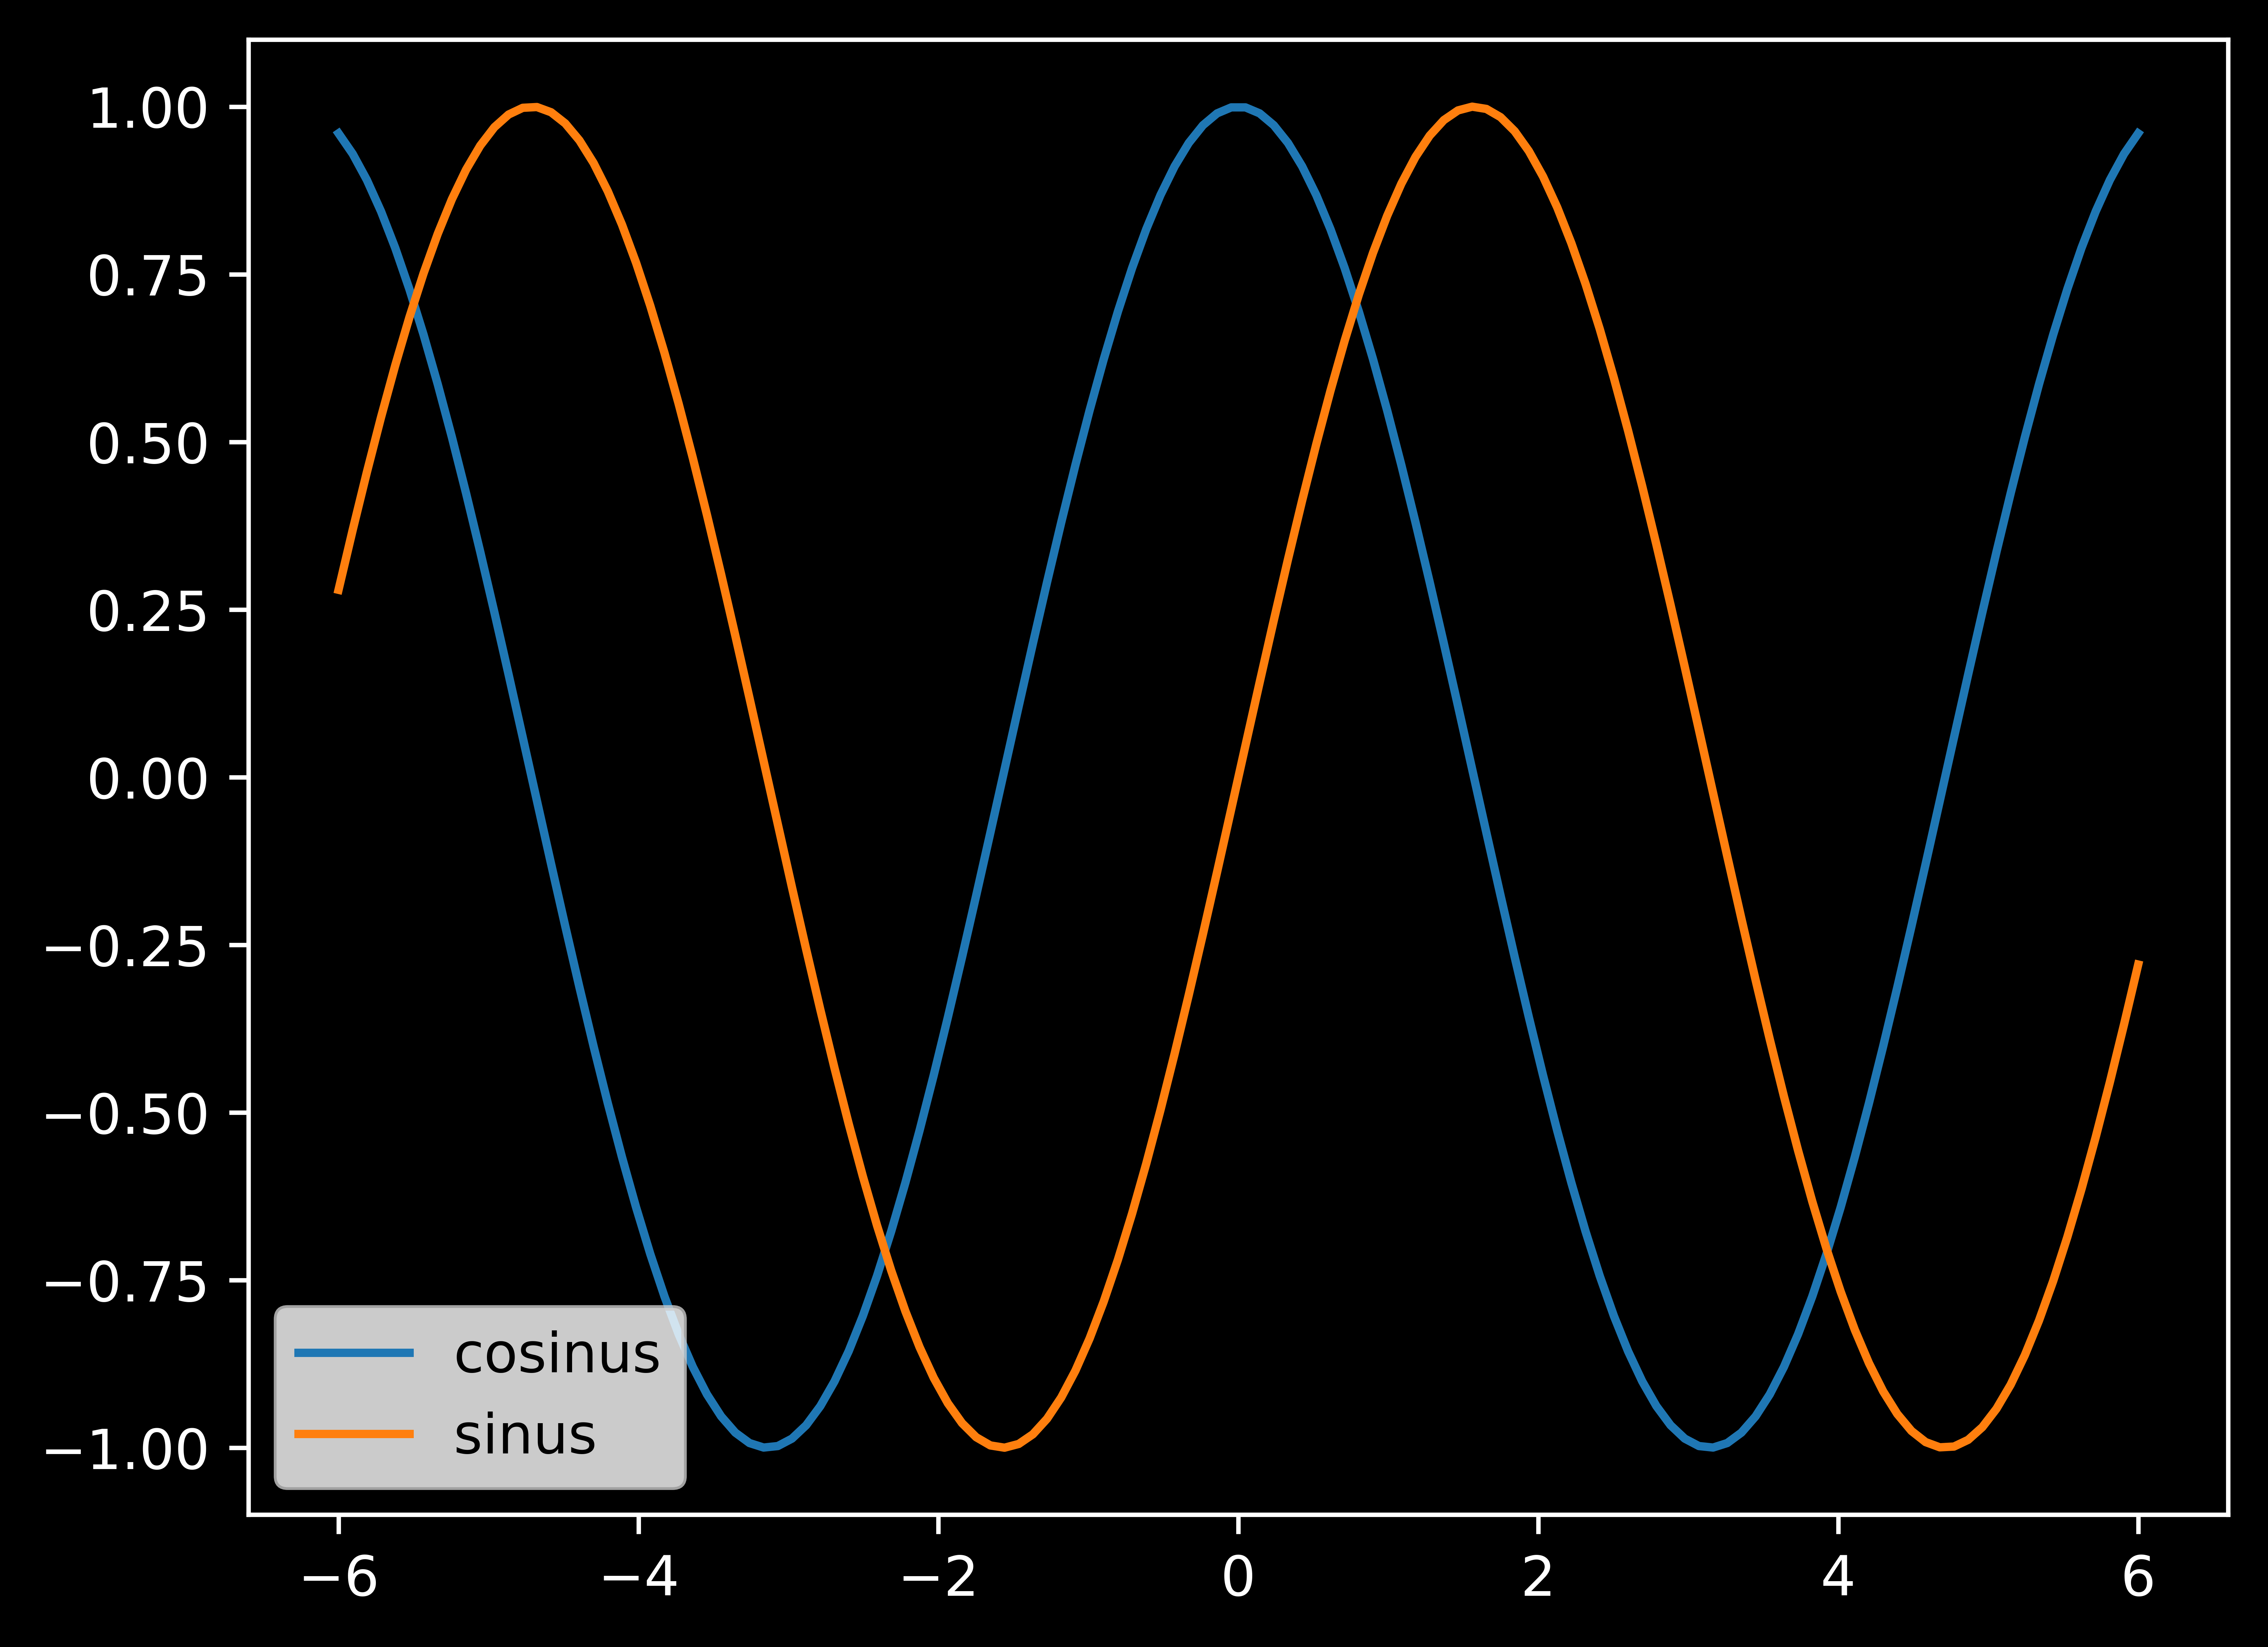
\includegraphics[width=\textwidth]{mline_plot_legend}
  \end{minipage}
  \vfill
\end{frame}



\begin{frame}[fragile]{}{}
  \vfill
  \begin{minipage}{.48\textwidth}
    \begin{lstlisting}[language=Python]
      # Style d'une des courbes.
      plt.plot(
           x, y,
          label='cosinus')
      plt.plot(x, z,
          label='sinus',
          linestyle='--')
    \end{lstlisting}
  \end{minipage}%
  \hfill
  \begin{minipage}{.48\textwidth}
    \centering
    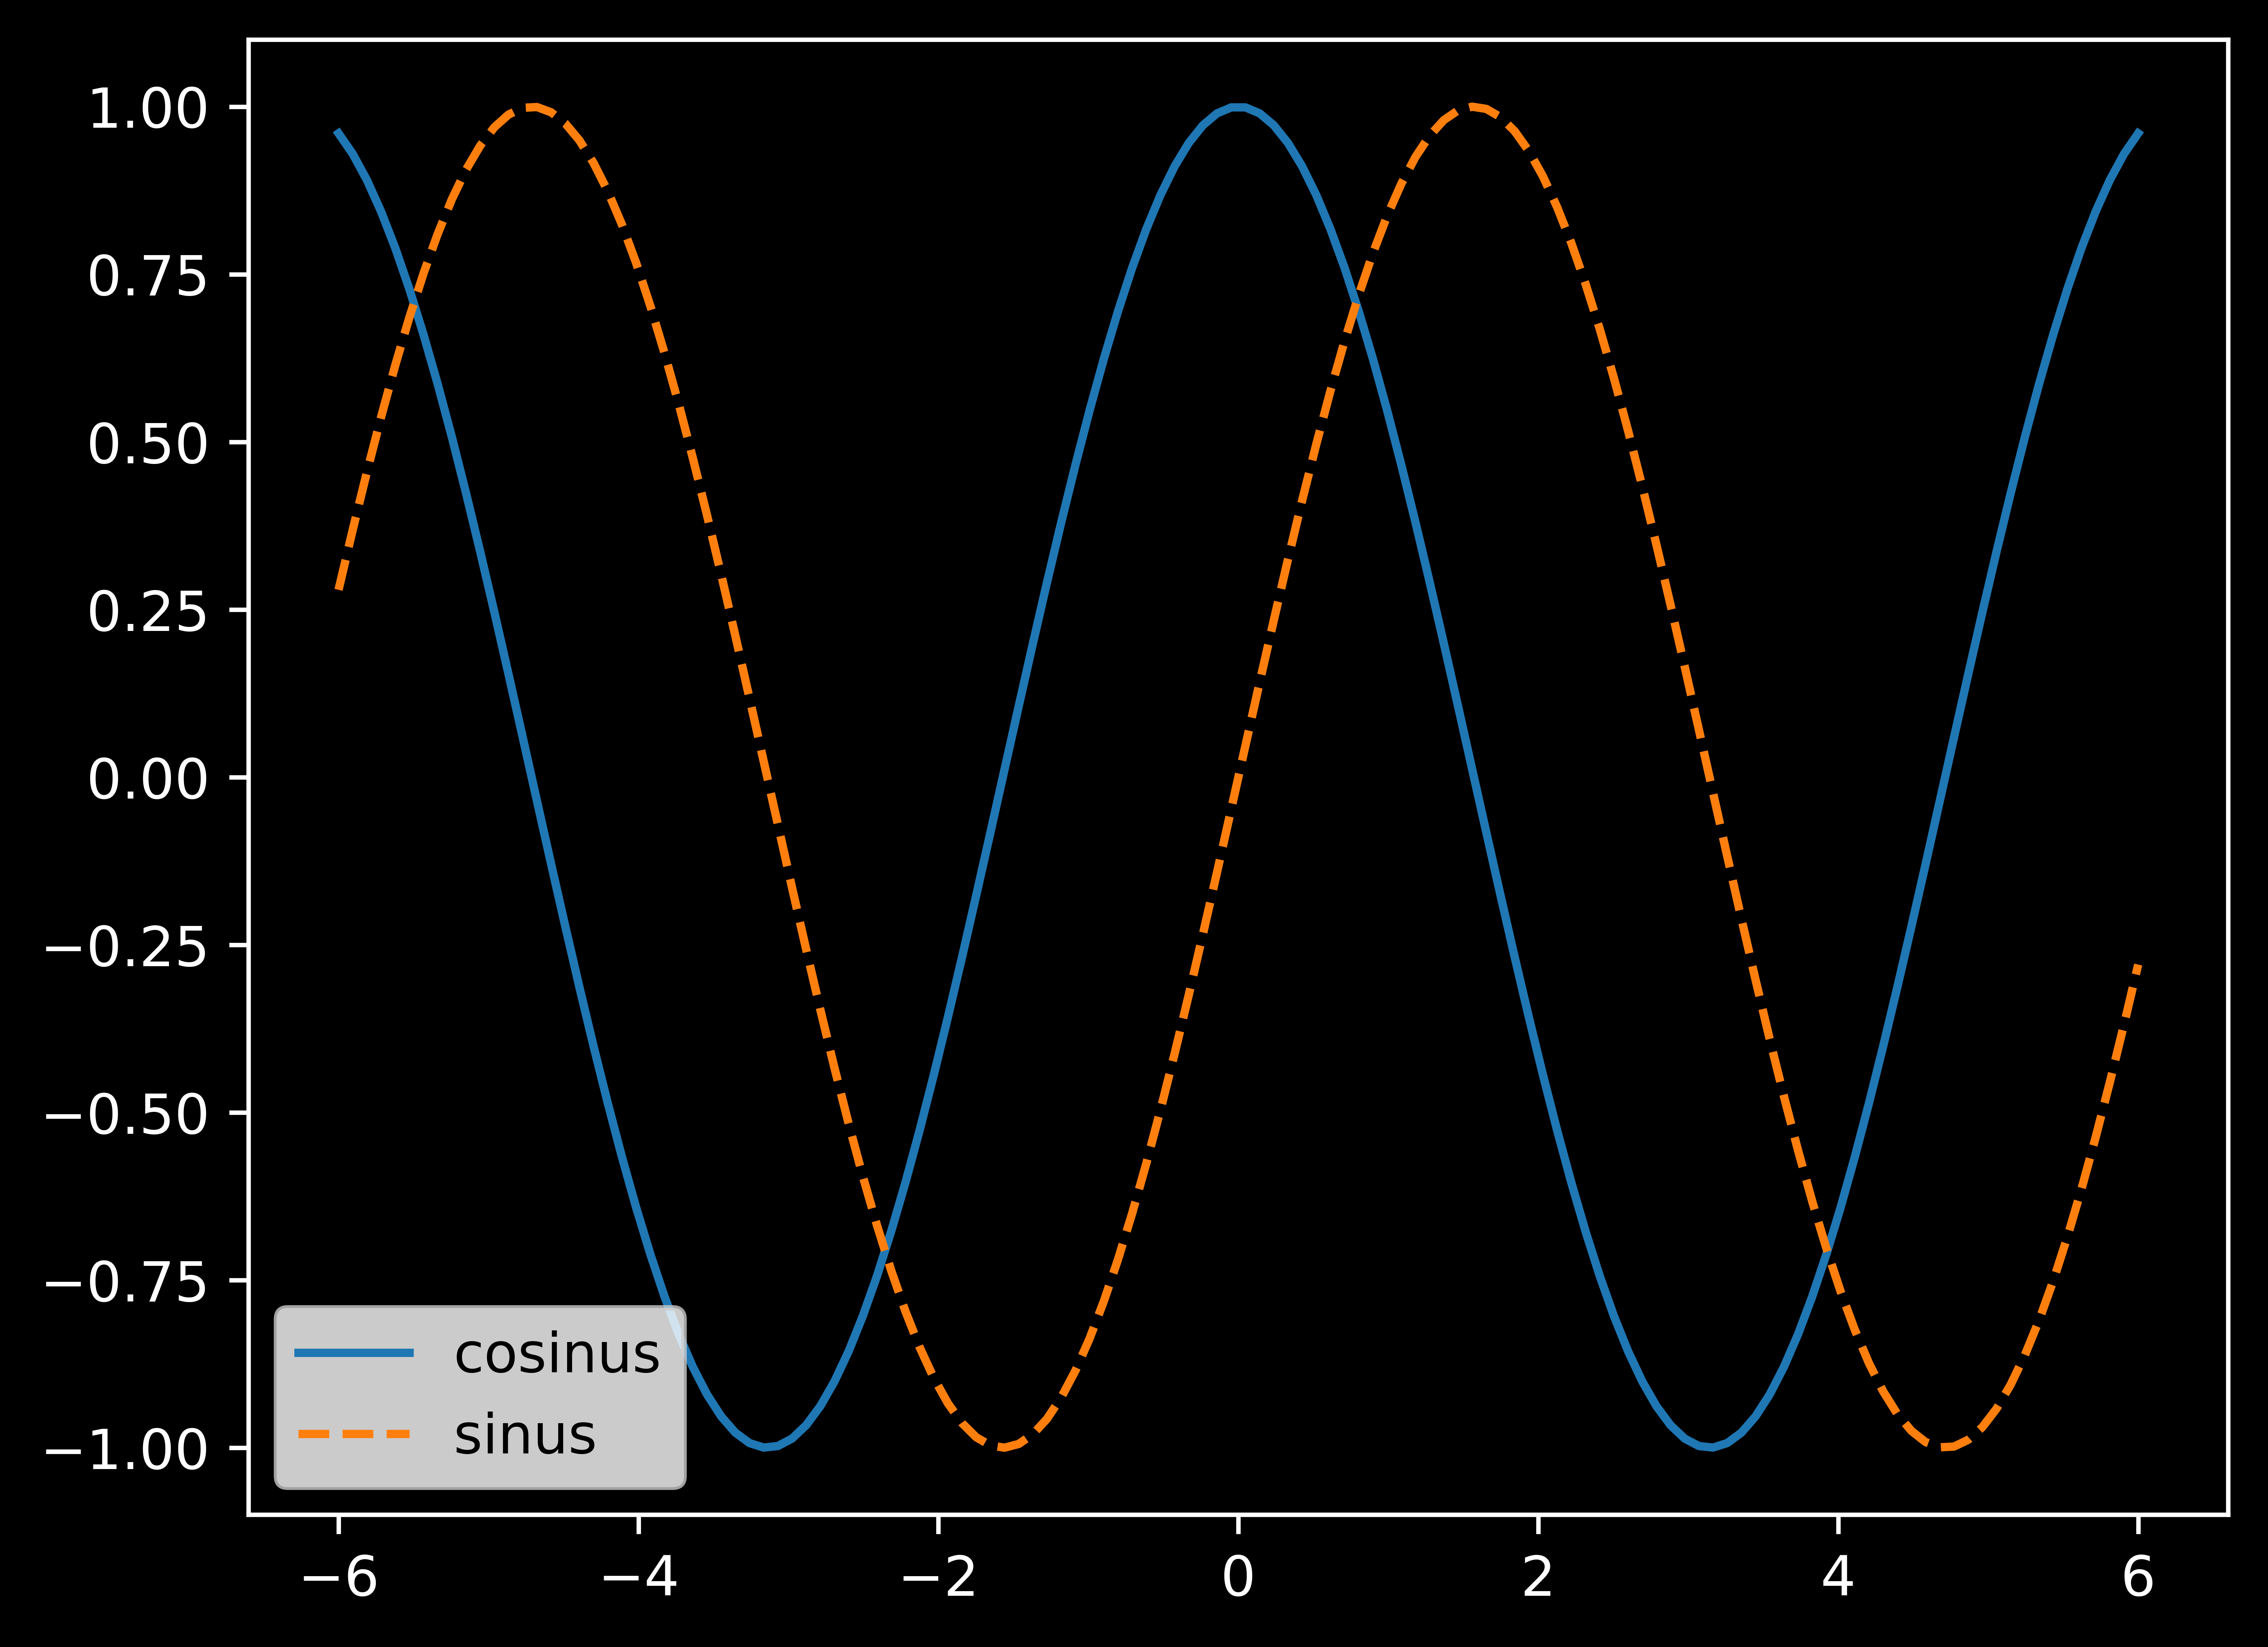
\includegraphics[width=\textwidth]{mline_plot_style}
  \end{minipage}
  \vfill
\end{frame}

\frame{}

\begin{frame}[fragile]{}{}
  \vfill
  \begin{minipage}{.48\textwidth}
    \begin{lstlisting}[language=Python]
      # Donnees synthetiques.
      x = np.linspace(0, 10, 128)
      y = np.exp(x)

      # Cree la figure.
      plt.figure()

      # Plot par defaut.
      plt.plot(x, y)

      plt.show()
    \end{lstlisting}
  \end{minipage}%
  \hfill
  \begin{minipage}{.48\textwidth}
    \centering
    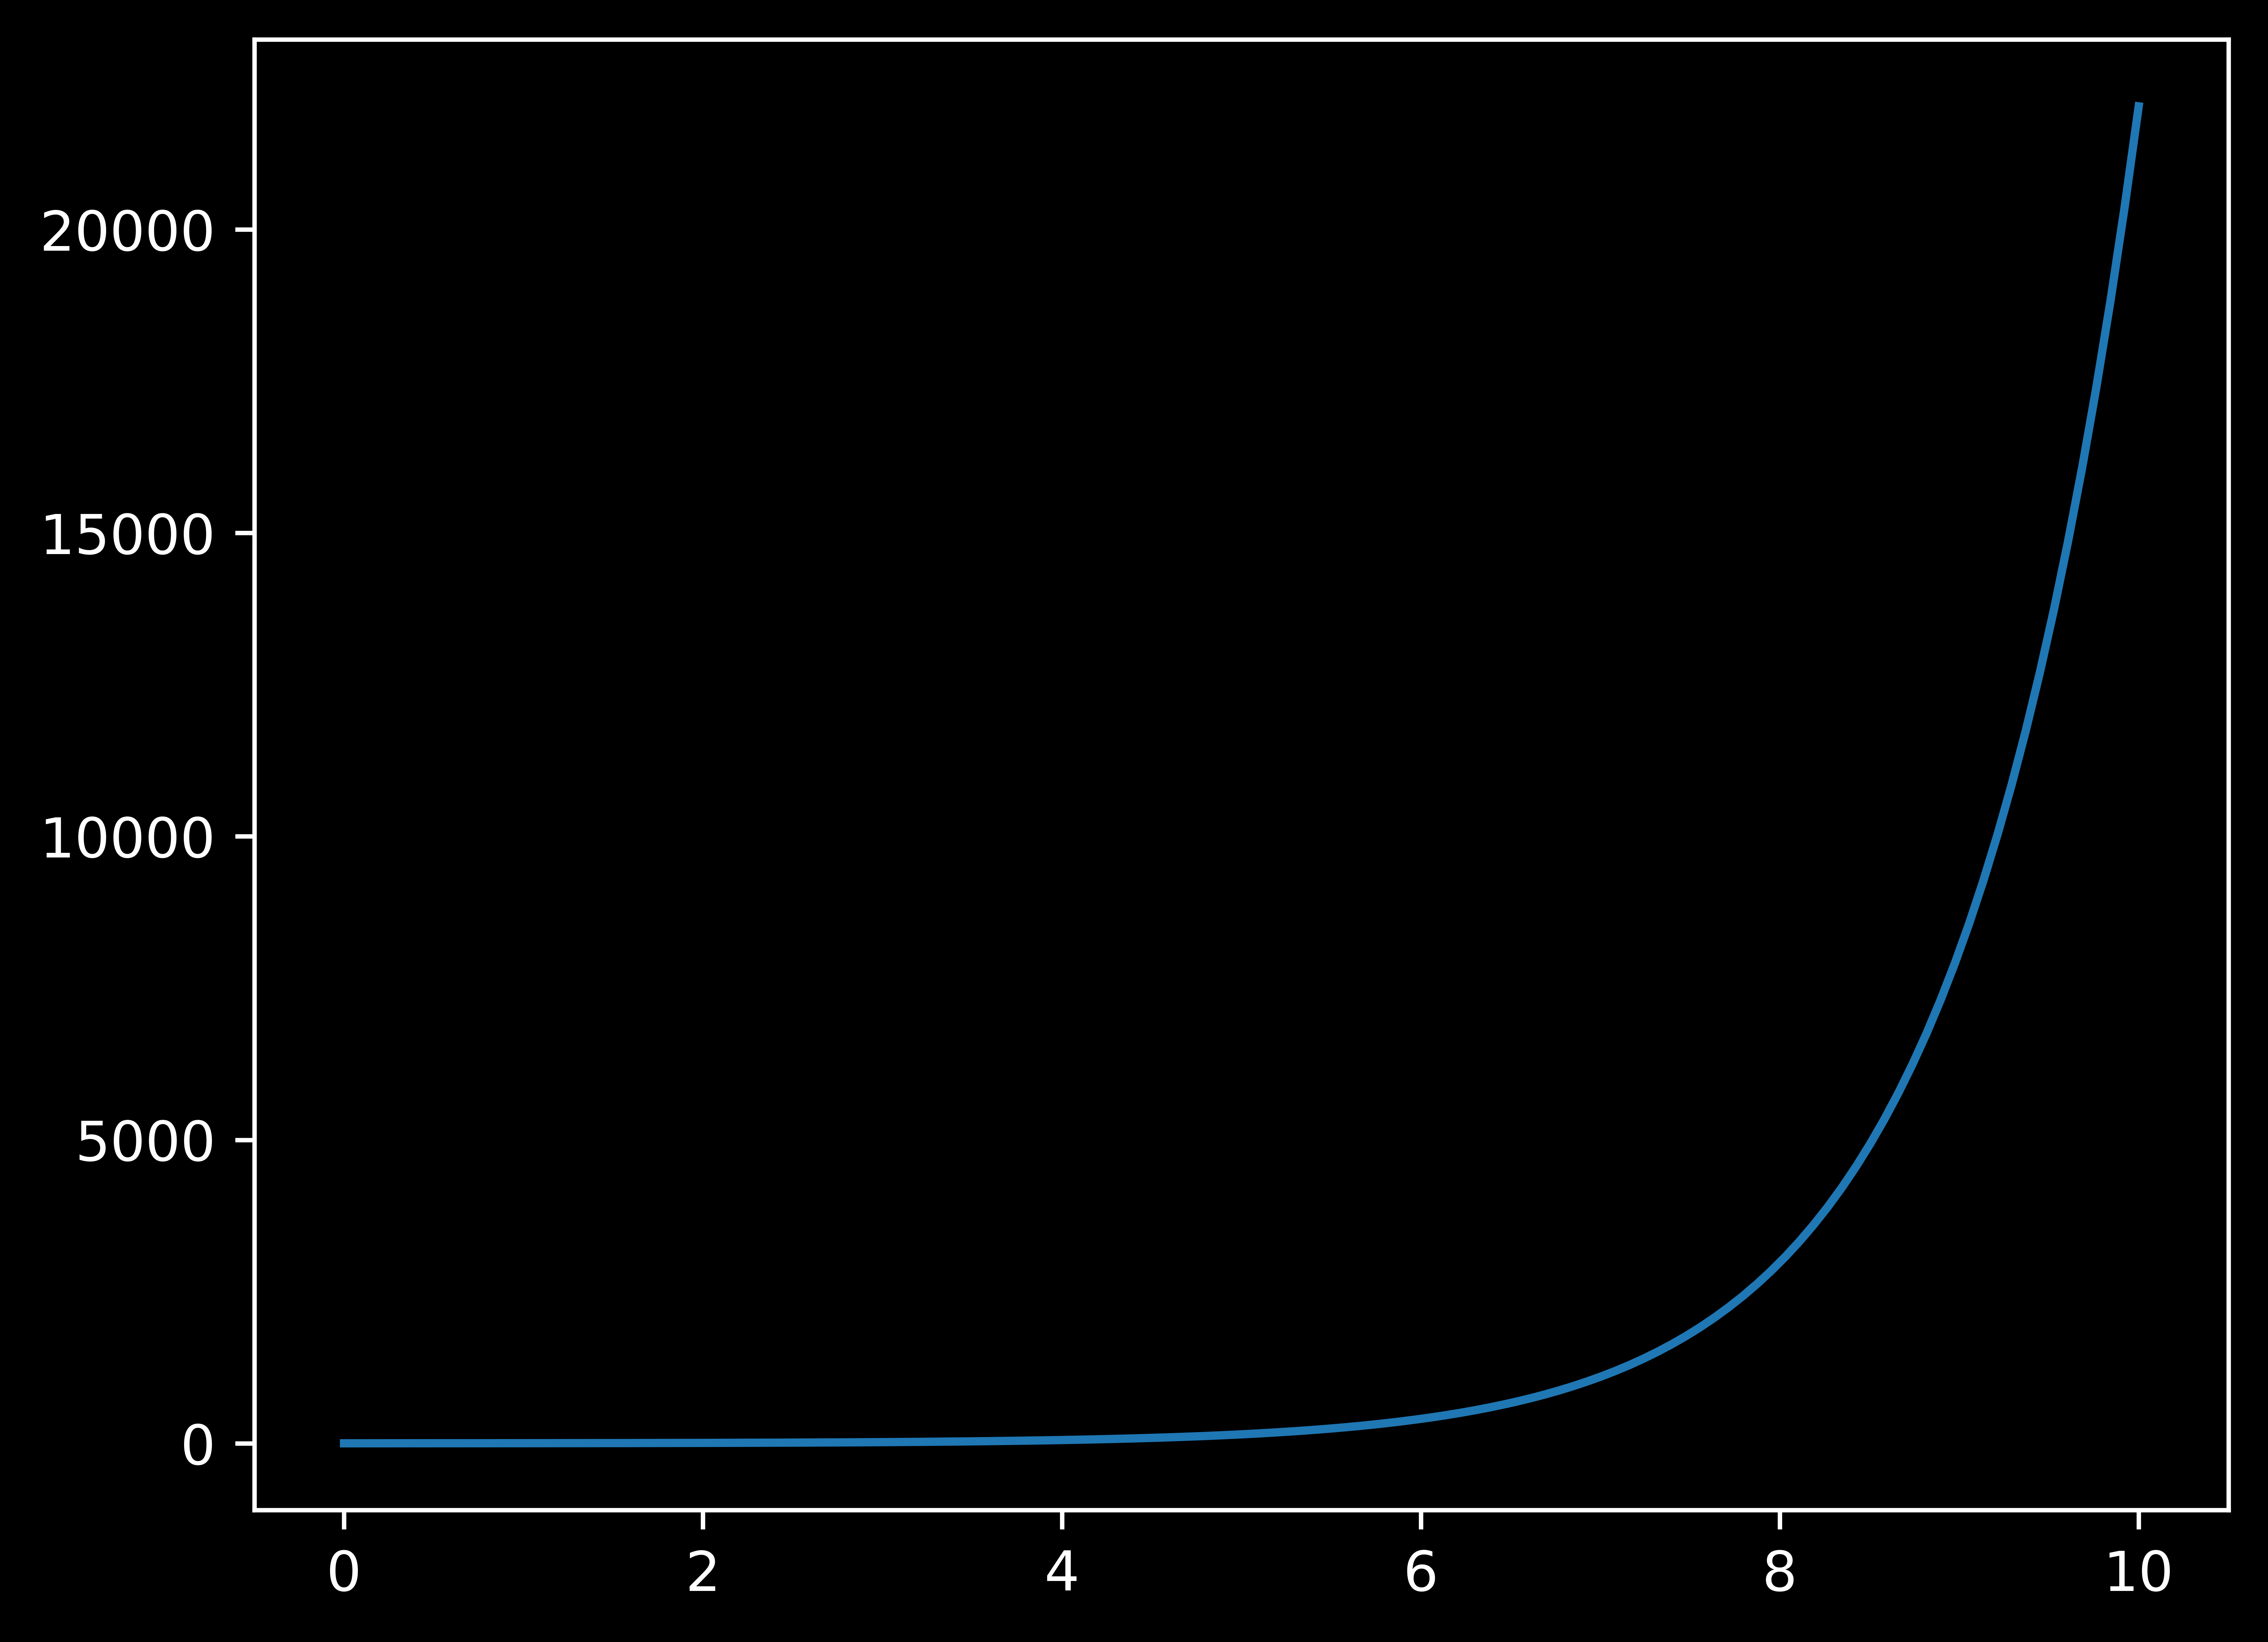
\includegraphics[width=\textwidth]{scale_line_plot_default}
  \end{minipage}
  \vfill
\end{frame}





\begin{frame}[fragile]{}{}
  \vfill
  \begin{minipage}{.48\textwidth}
    \begin{lstlisting}[language=Python]

      # Echelle log en x.
      plt.semilogx(x, y)

      # Echelle log en y.
      plt.semilogy(x, y)

      # Echelle log-log.
      plt.loglog(x, y)
    \end{lstlisting}
  \end{minipage}%
  \hfill
  \begin{minipage}{.48\textwidth}
    \centering
    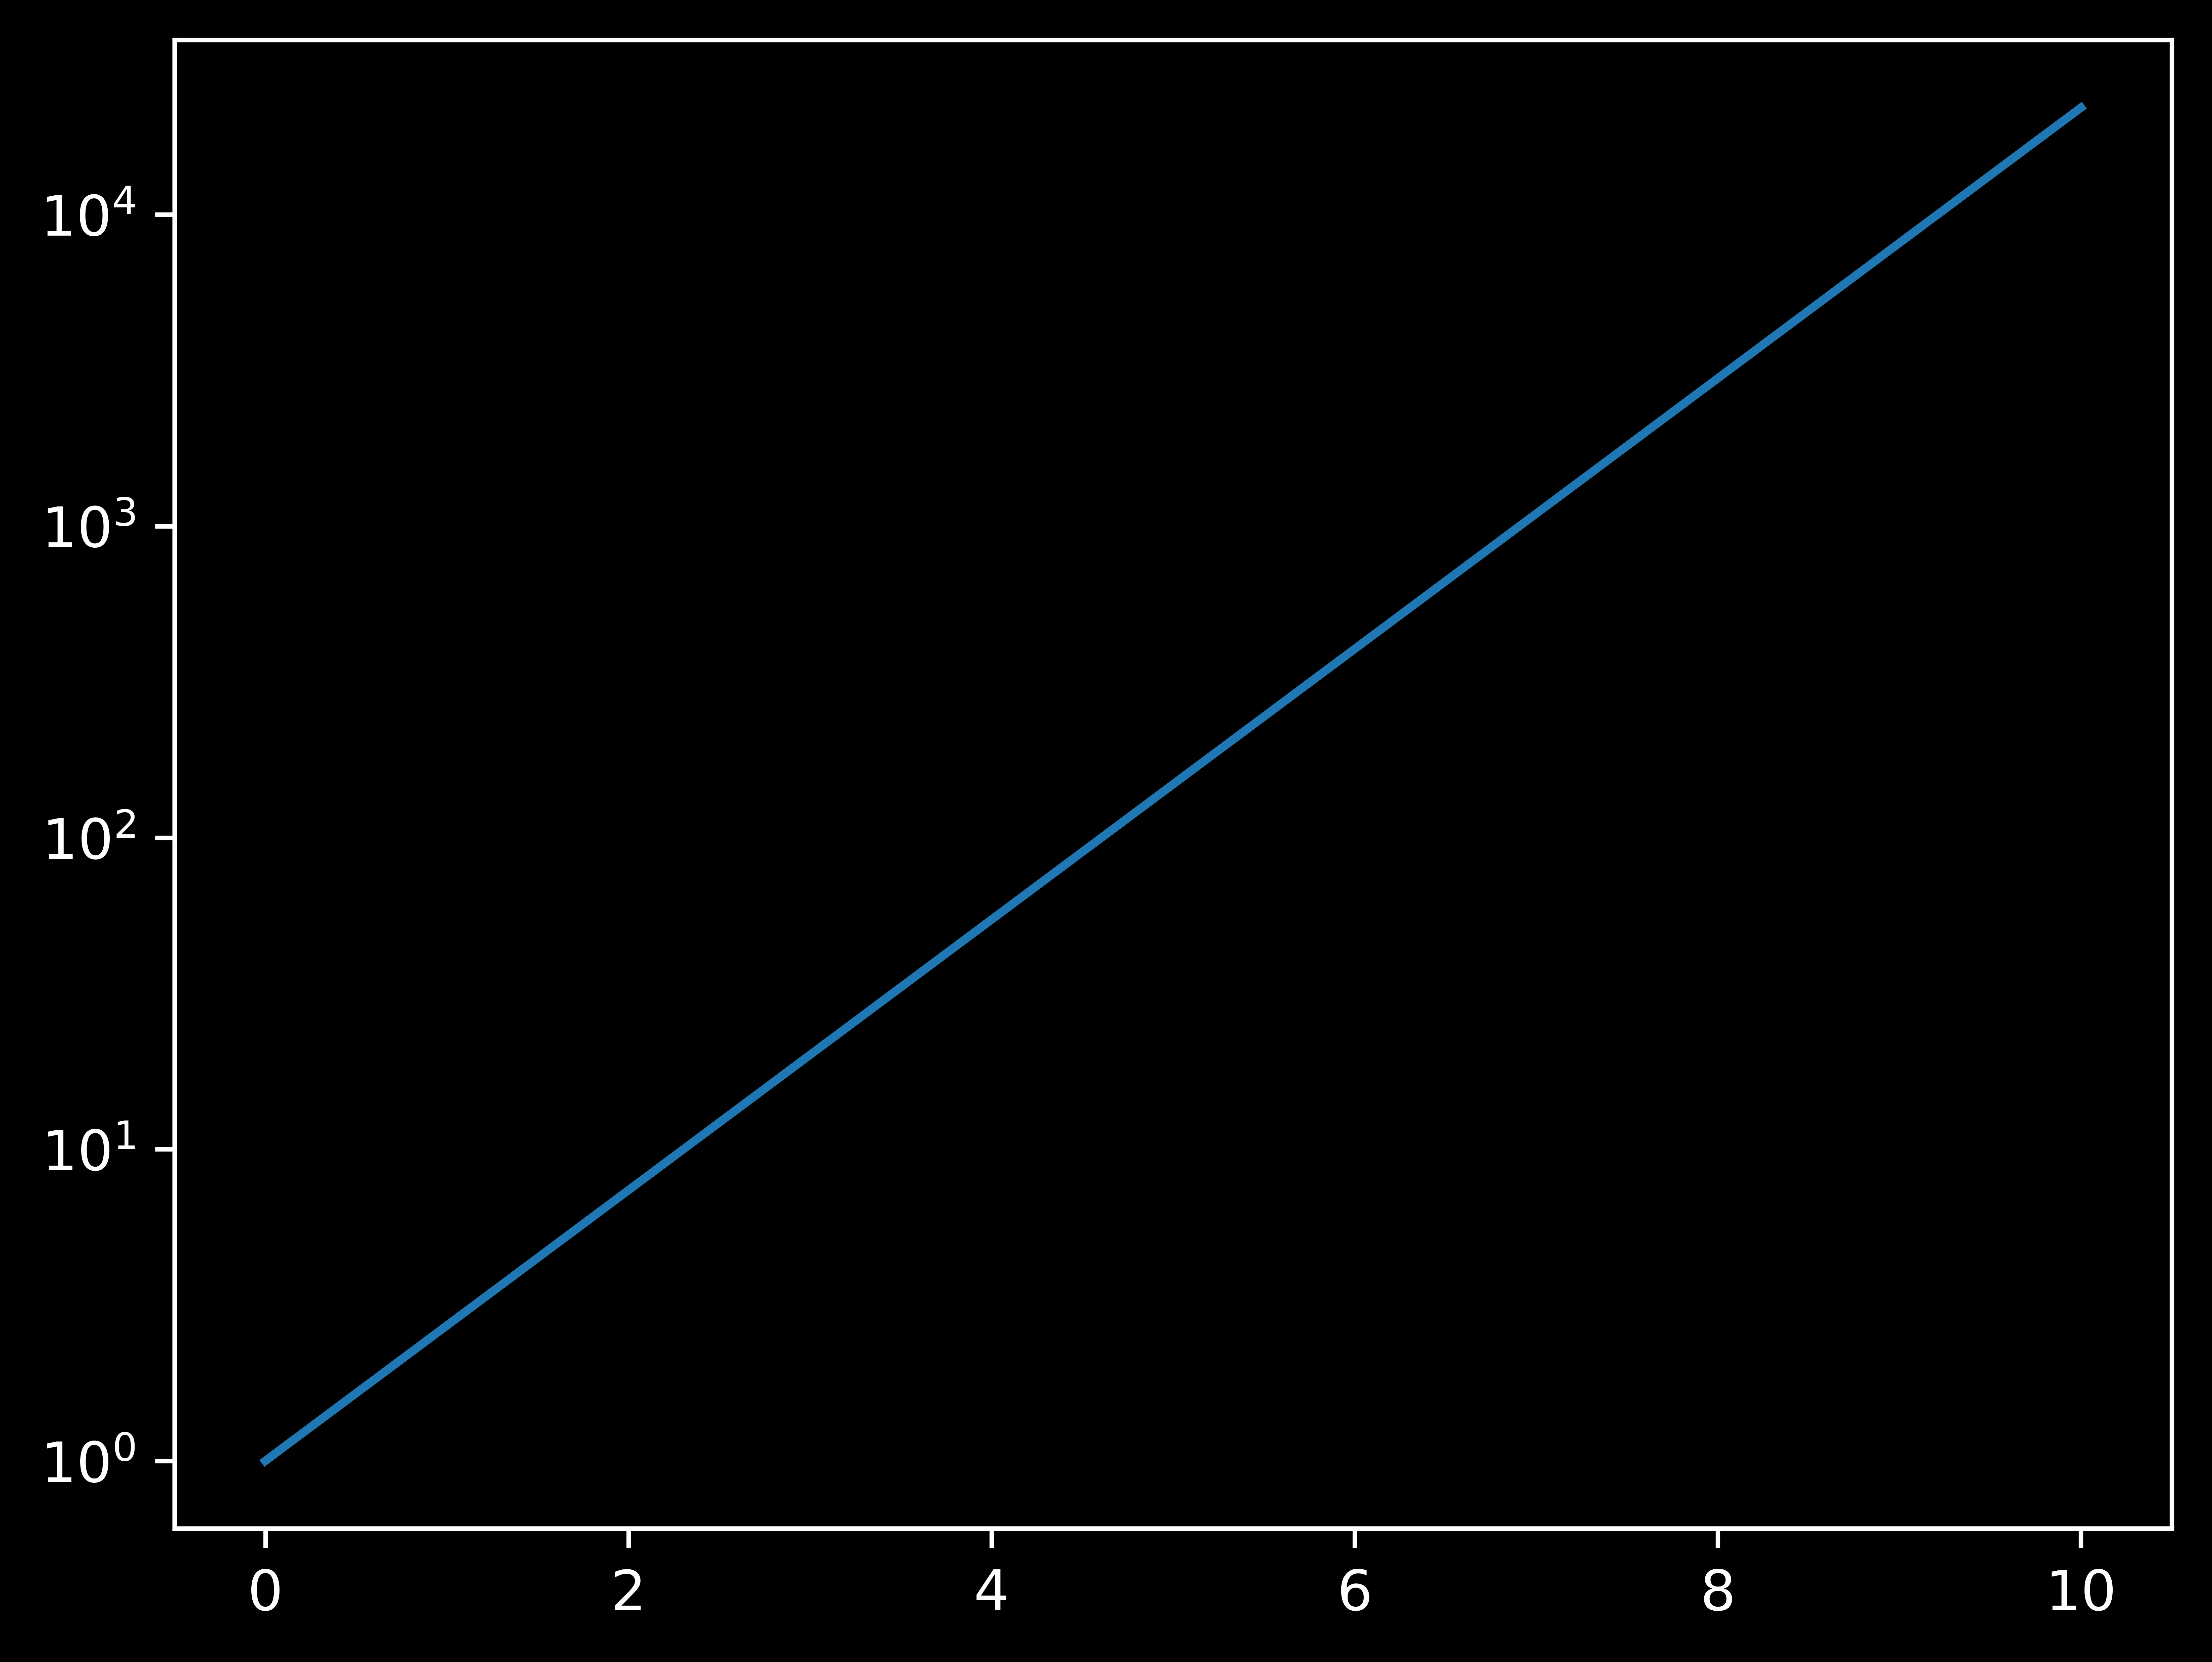
\includegraphics[width=\textwidth]{scale_line_plot_logy}
  \end{minipage}
  \vfill
\end{frame}





\begin{frame}
  \vfill
  \centering
  \textbf{Tracer des nuages de points}
  \vfill
\end{frame}


{
  \setbeamercolor{background canvas}{bg=white}
  \frame{
    \vfill
    \centering
    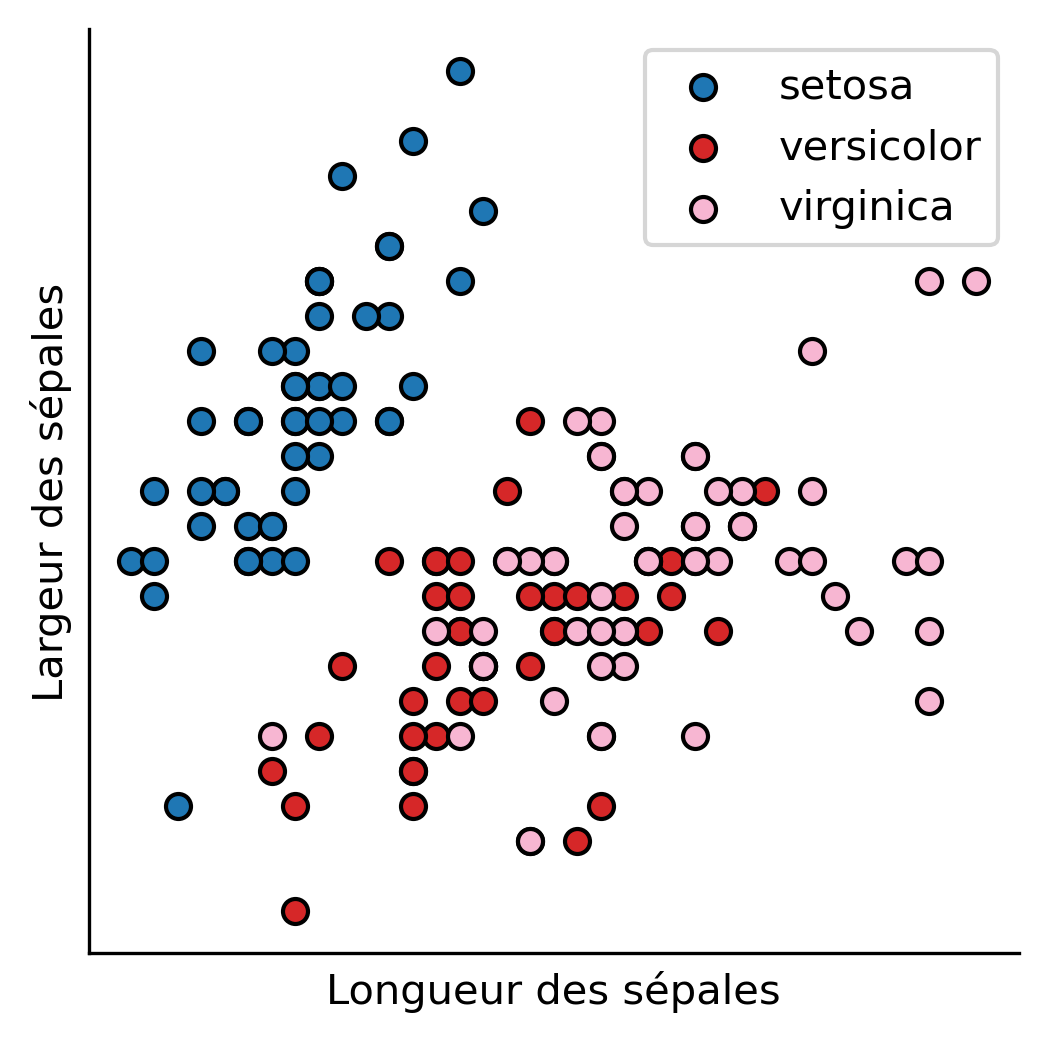
\includegraphics[height=.8\textheight]{iris_dataset}
    \vfill
  }
}

\begin{frame}[fragile]{}{}
  \vfill
  \begin{minipage}{.48\textwidth}
    \begin{lstlisting}[language=Python]
      # Donnees synthetiques.
      x = npr.randn(20, 2)

      # Cree la figure.
      plt.figure()

      # Nuage de points.
      plt.scatter(
          x[:, 0], x[:, 1])

      plt.show()
    \end{lstlisting}
  \end{minipage}%
  \hfill
  \begin{minipage}{.48\textwidth}
    \centering
    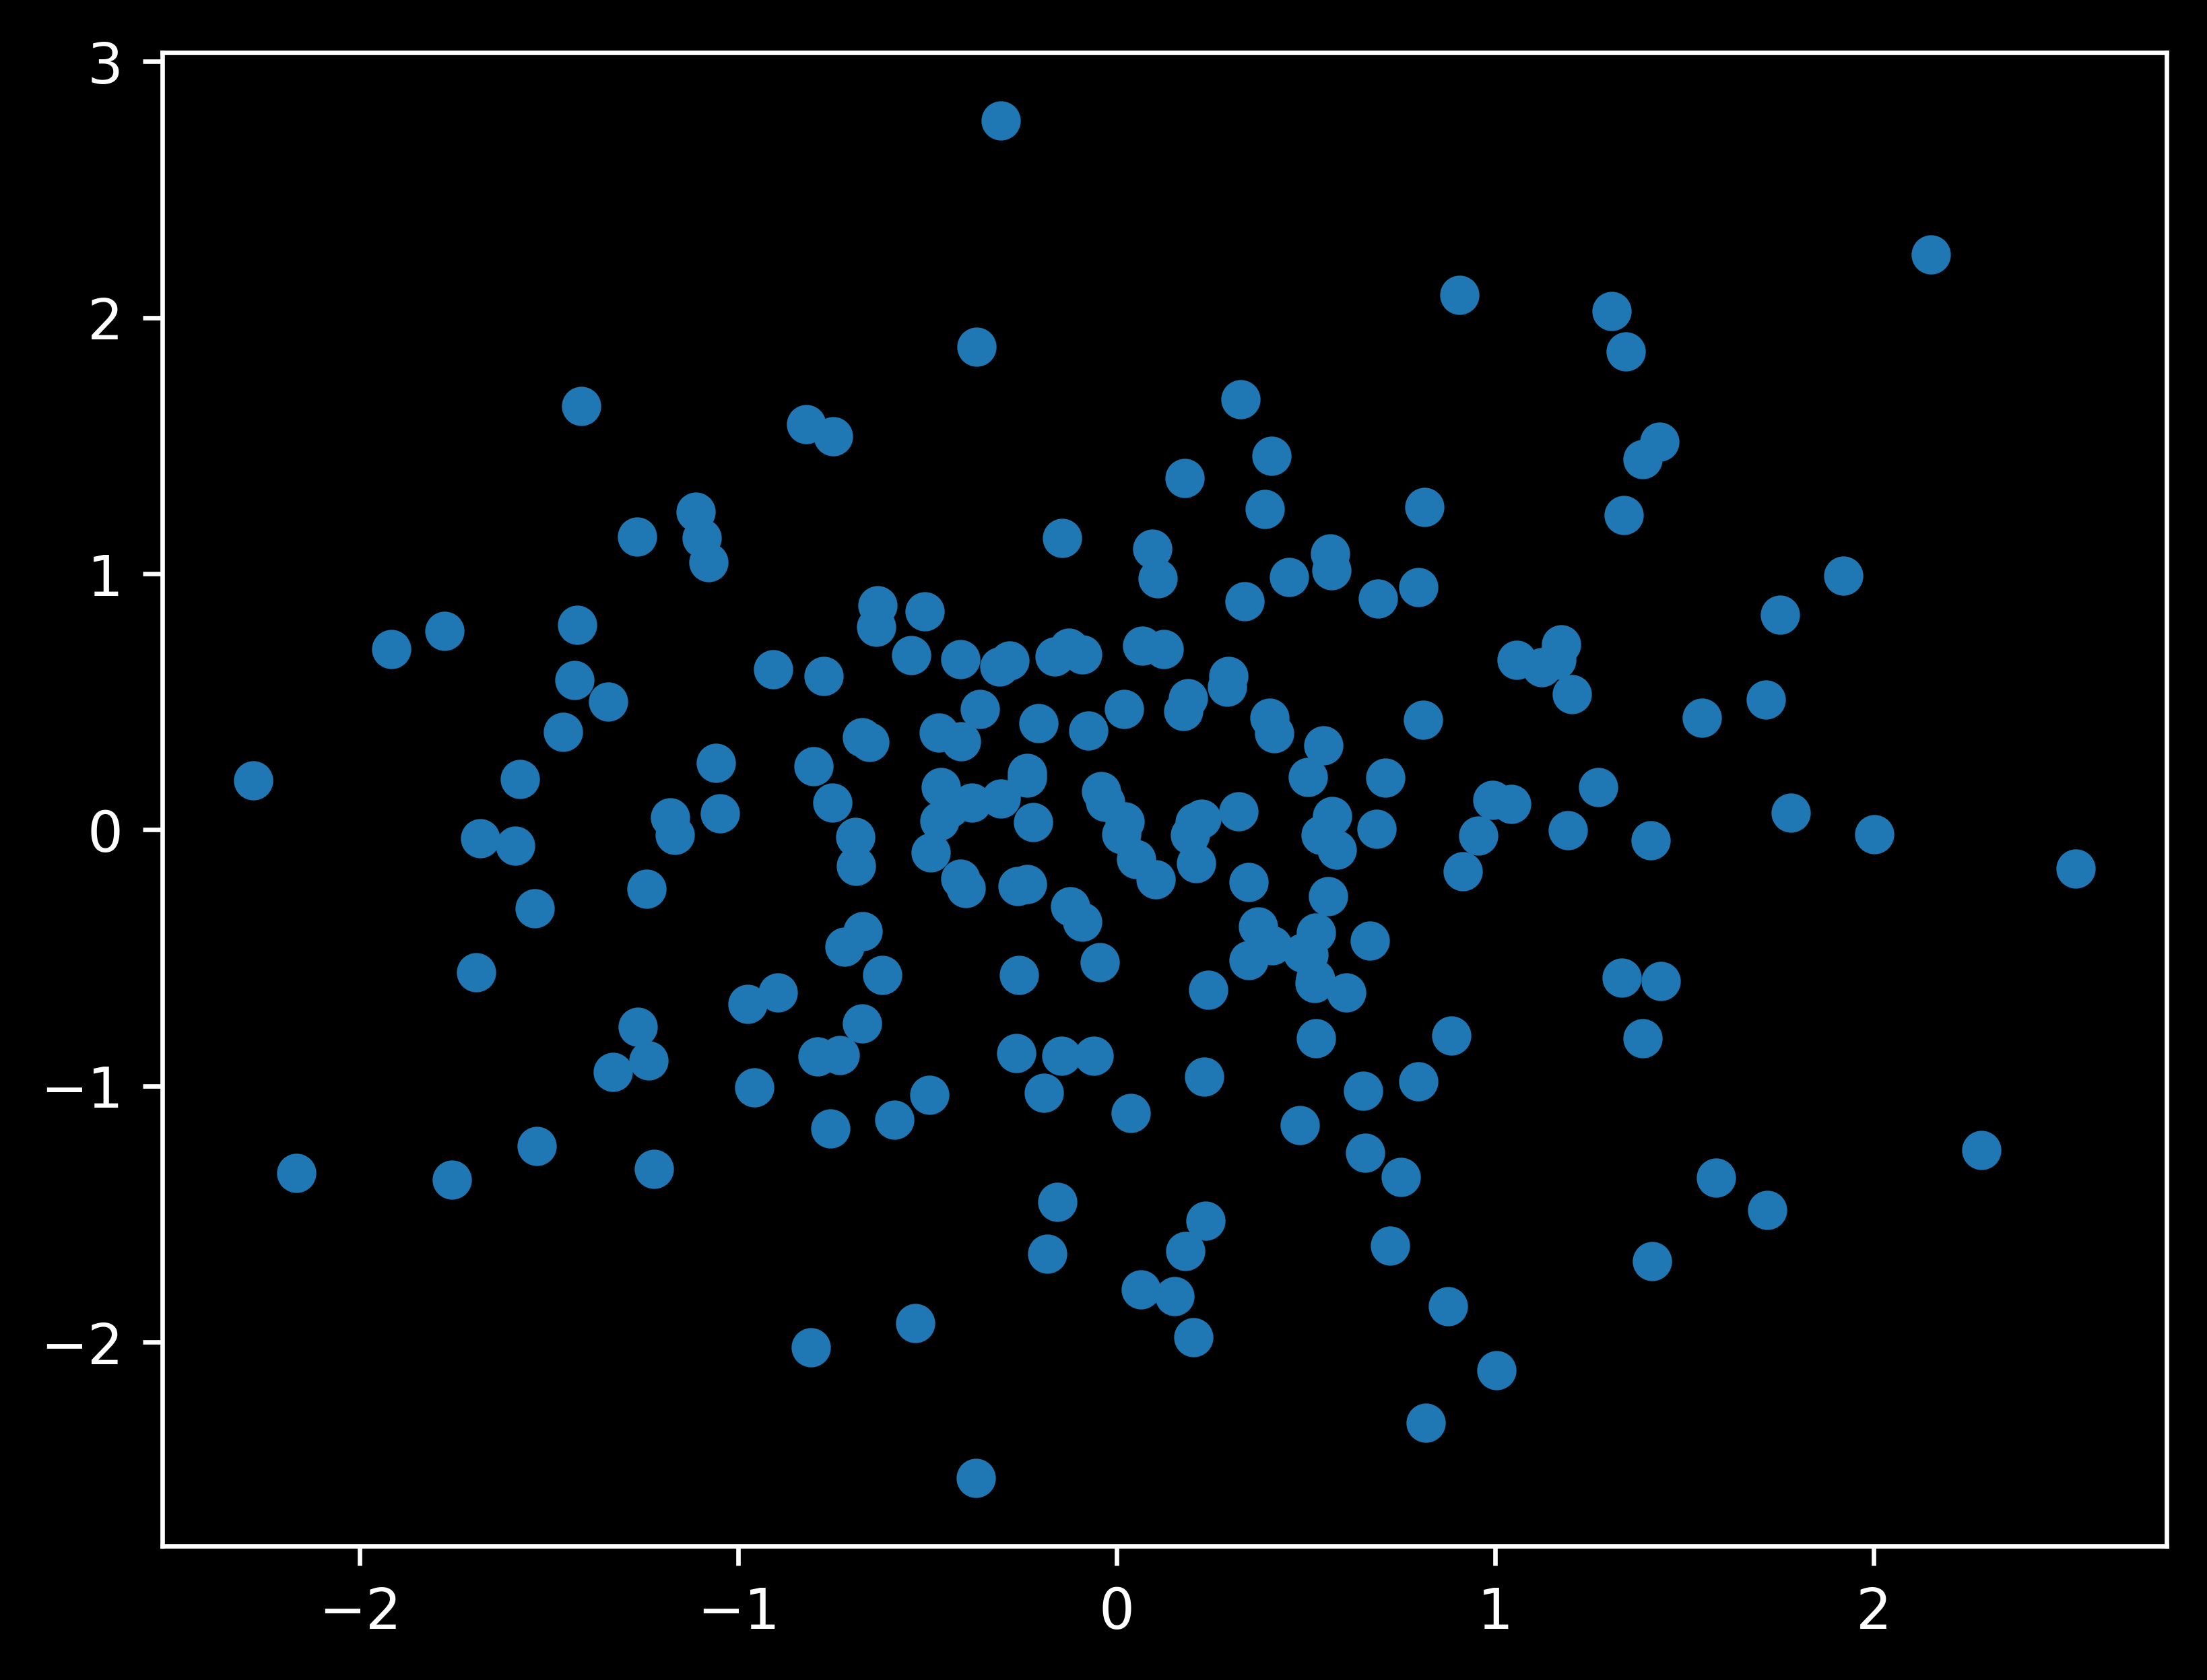
\includegraphics[width=\textwidth]{scatter_plot_default}
  \end{minipage}
  \vfill
\end{frame}



\begin{frame}[fragile]{}{}
  \vfill
  \begin{minipage}{.48\textwidth}
    \begin{lstlisting}[language=Python]
      # Transparence.
      plt.scatter(
          x[:, 0], x[:, 1],
          alpha=0.5)
    \end{lstlisting}
  \end{minipage}%
  \hfill
  \begin{minipage}{.48\textwidth}
    \centering
    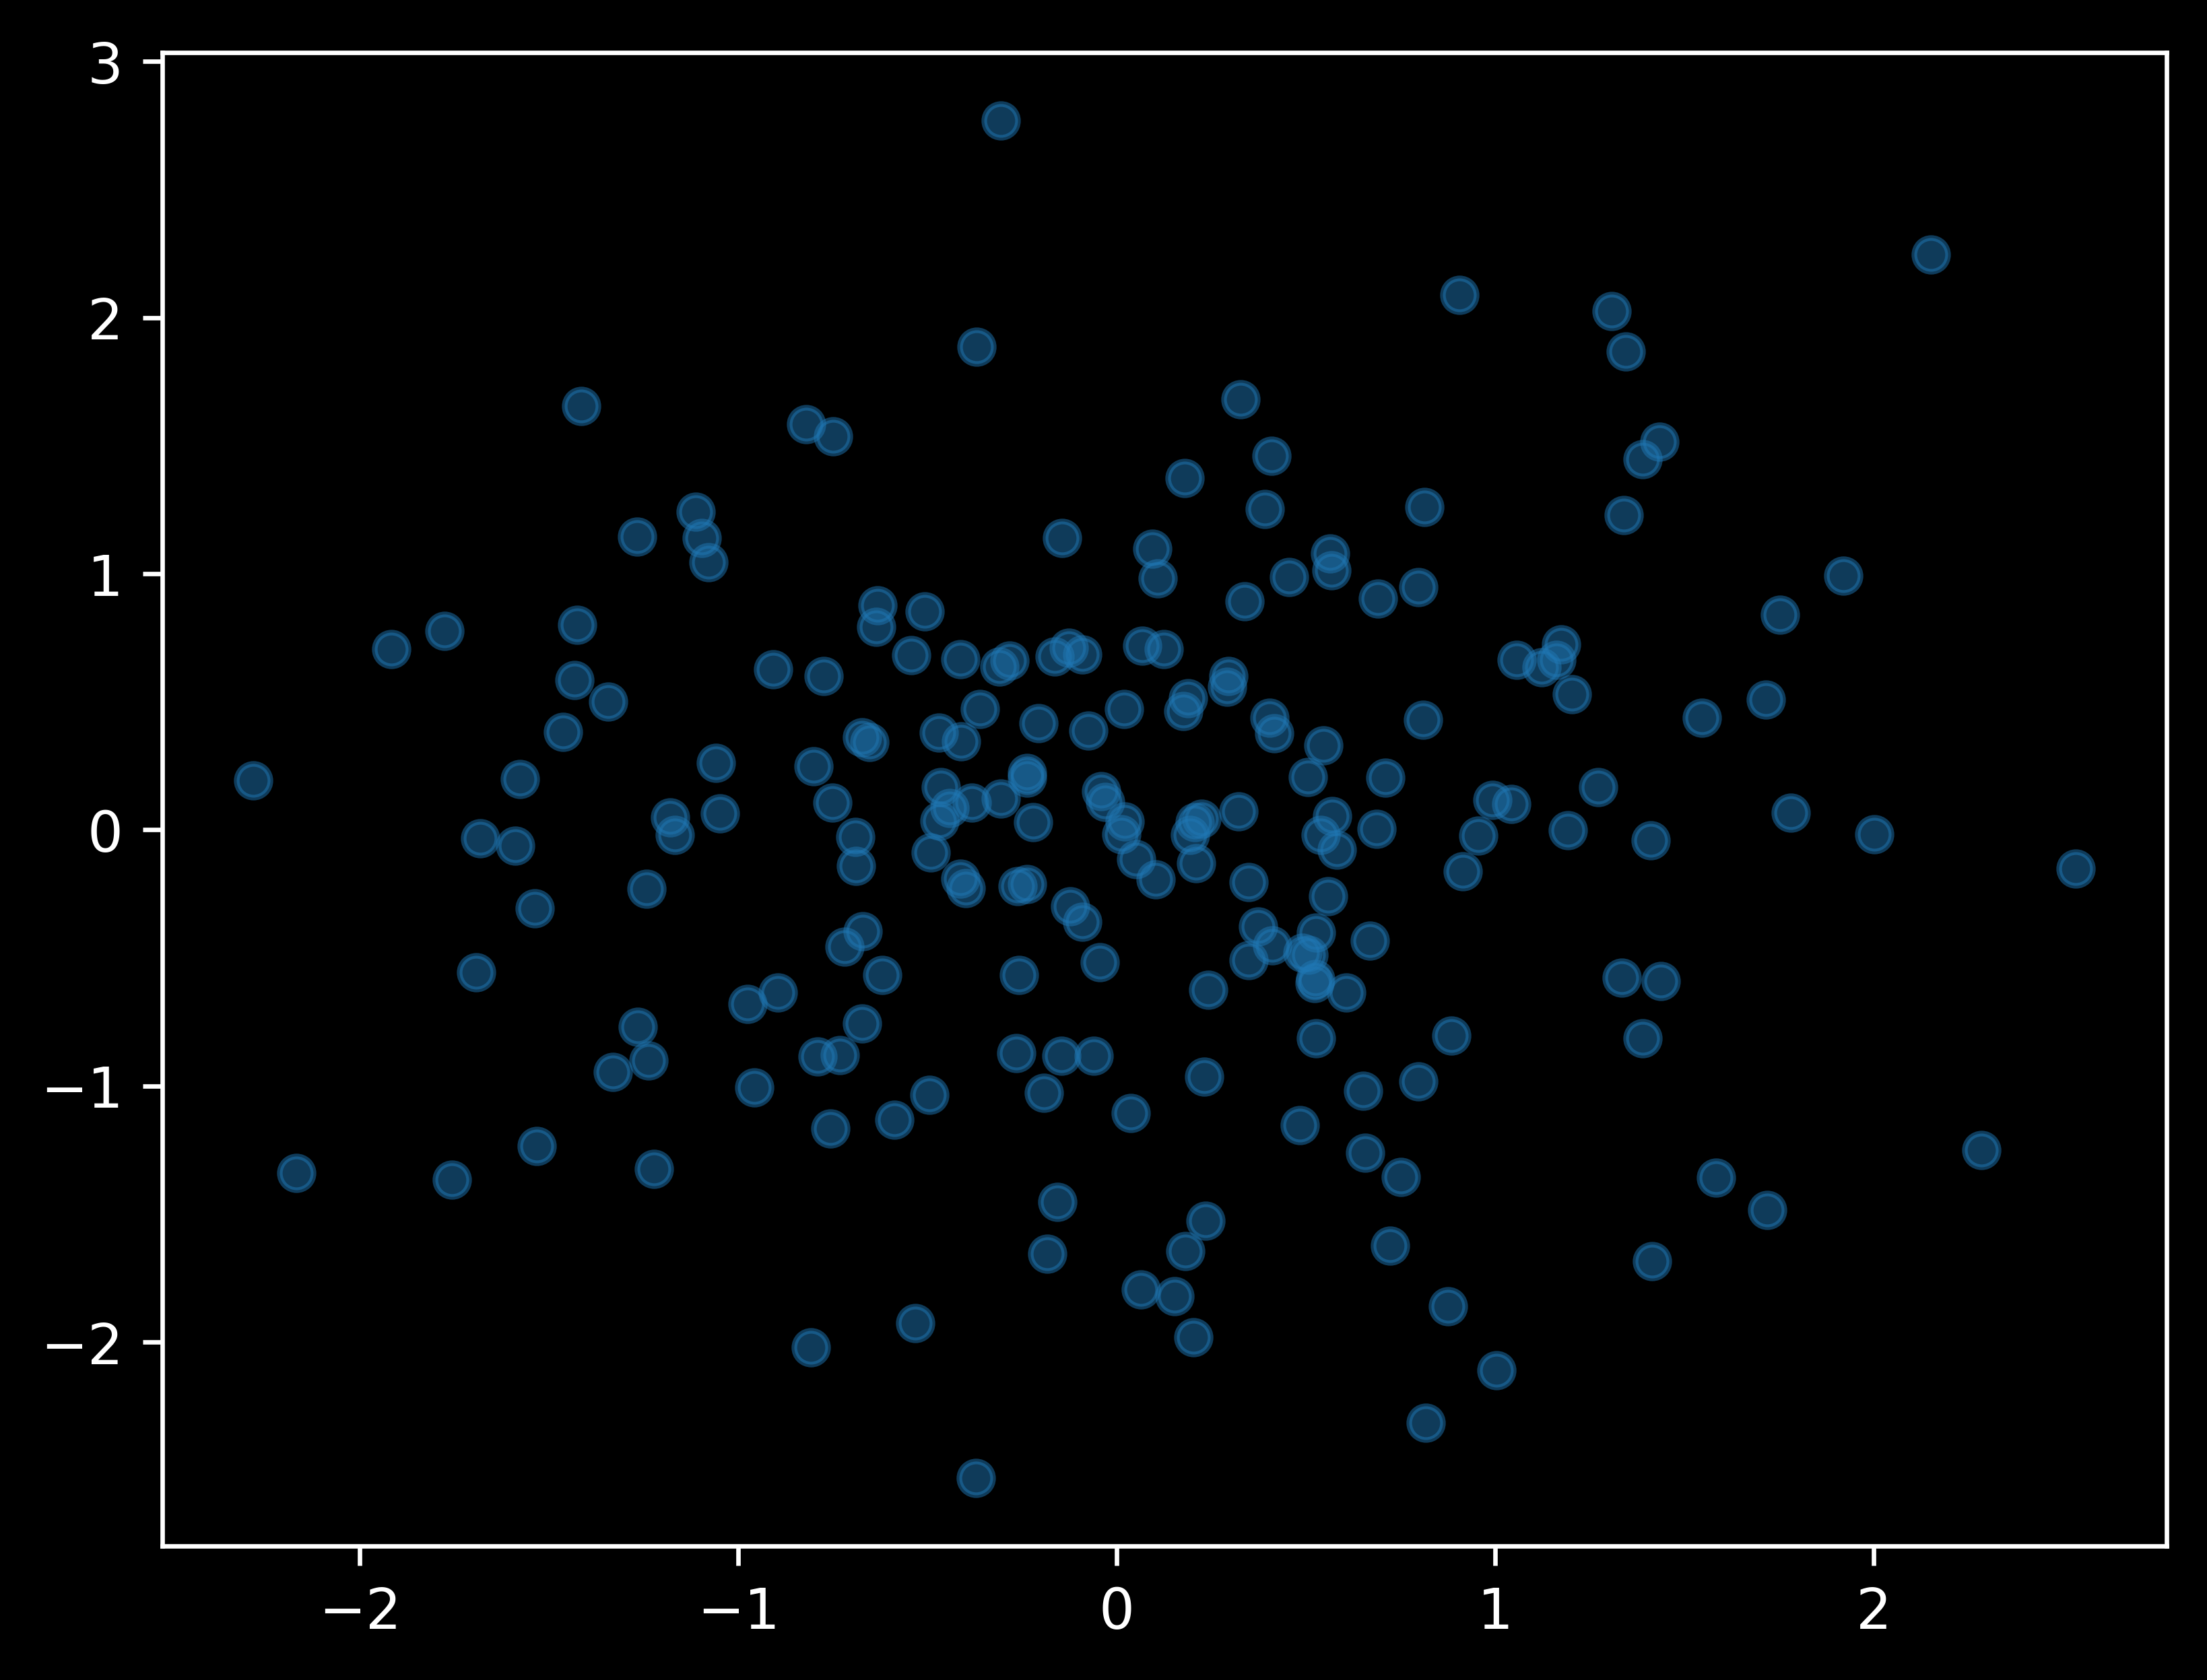
\includegraphics[width=\textwidth]{scatter_plot_alpha}
  \end{minipage}
  \vfill
\end{frame}



\begin{frame}[fragile]{}{}
  \vfill
  \begin{minipage}{.48\textwidth}
    \begin{lstlisting}[language=Python]

      x = npr.randn(200, 2)
      y = npr.randn(200, 2) + 1

      # Nuage de points.
      plt.scatter(
          x[:, 0], x[:, 1],
          alpha=0.5)

      plt.scatter(
          y[:, 0], y[:, 1],
          alpha=0.5)
    \end{lstlisting}
  \end{minipage}%
  \hfill
  \begin{minipage}{.48\textwidth}
    \centering
    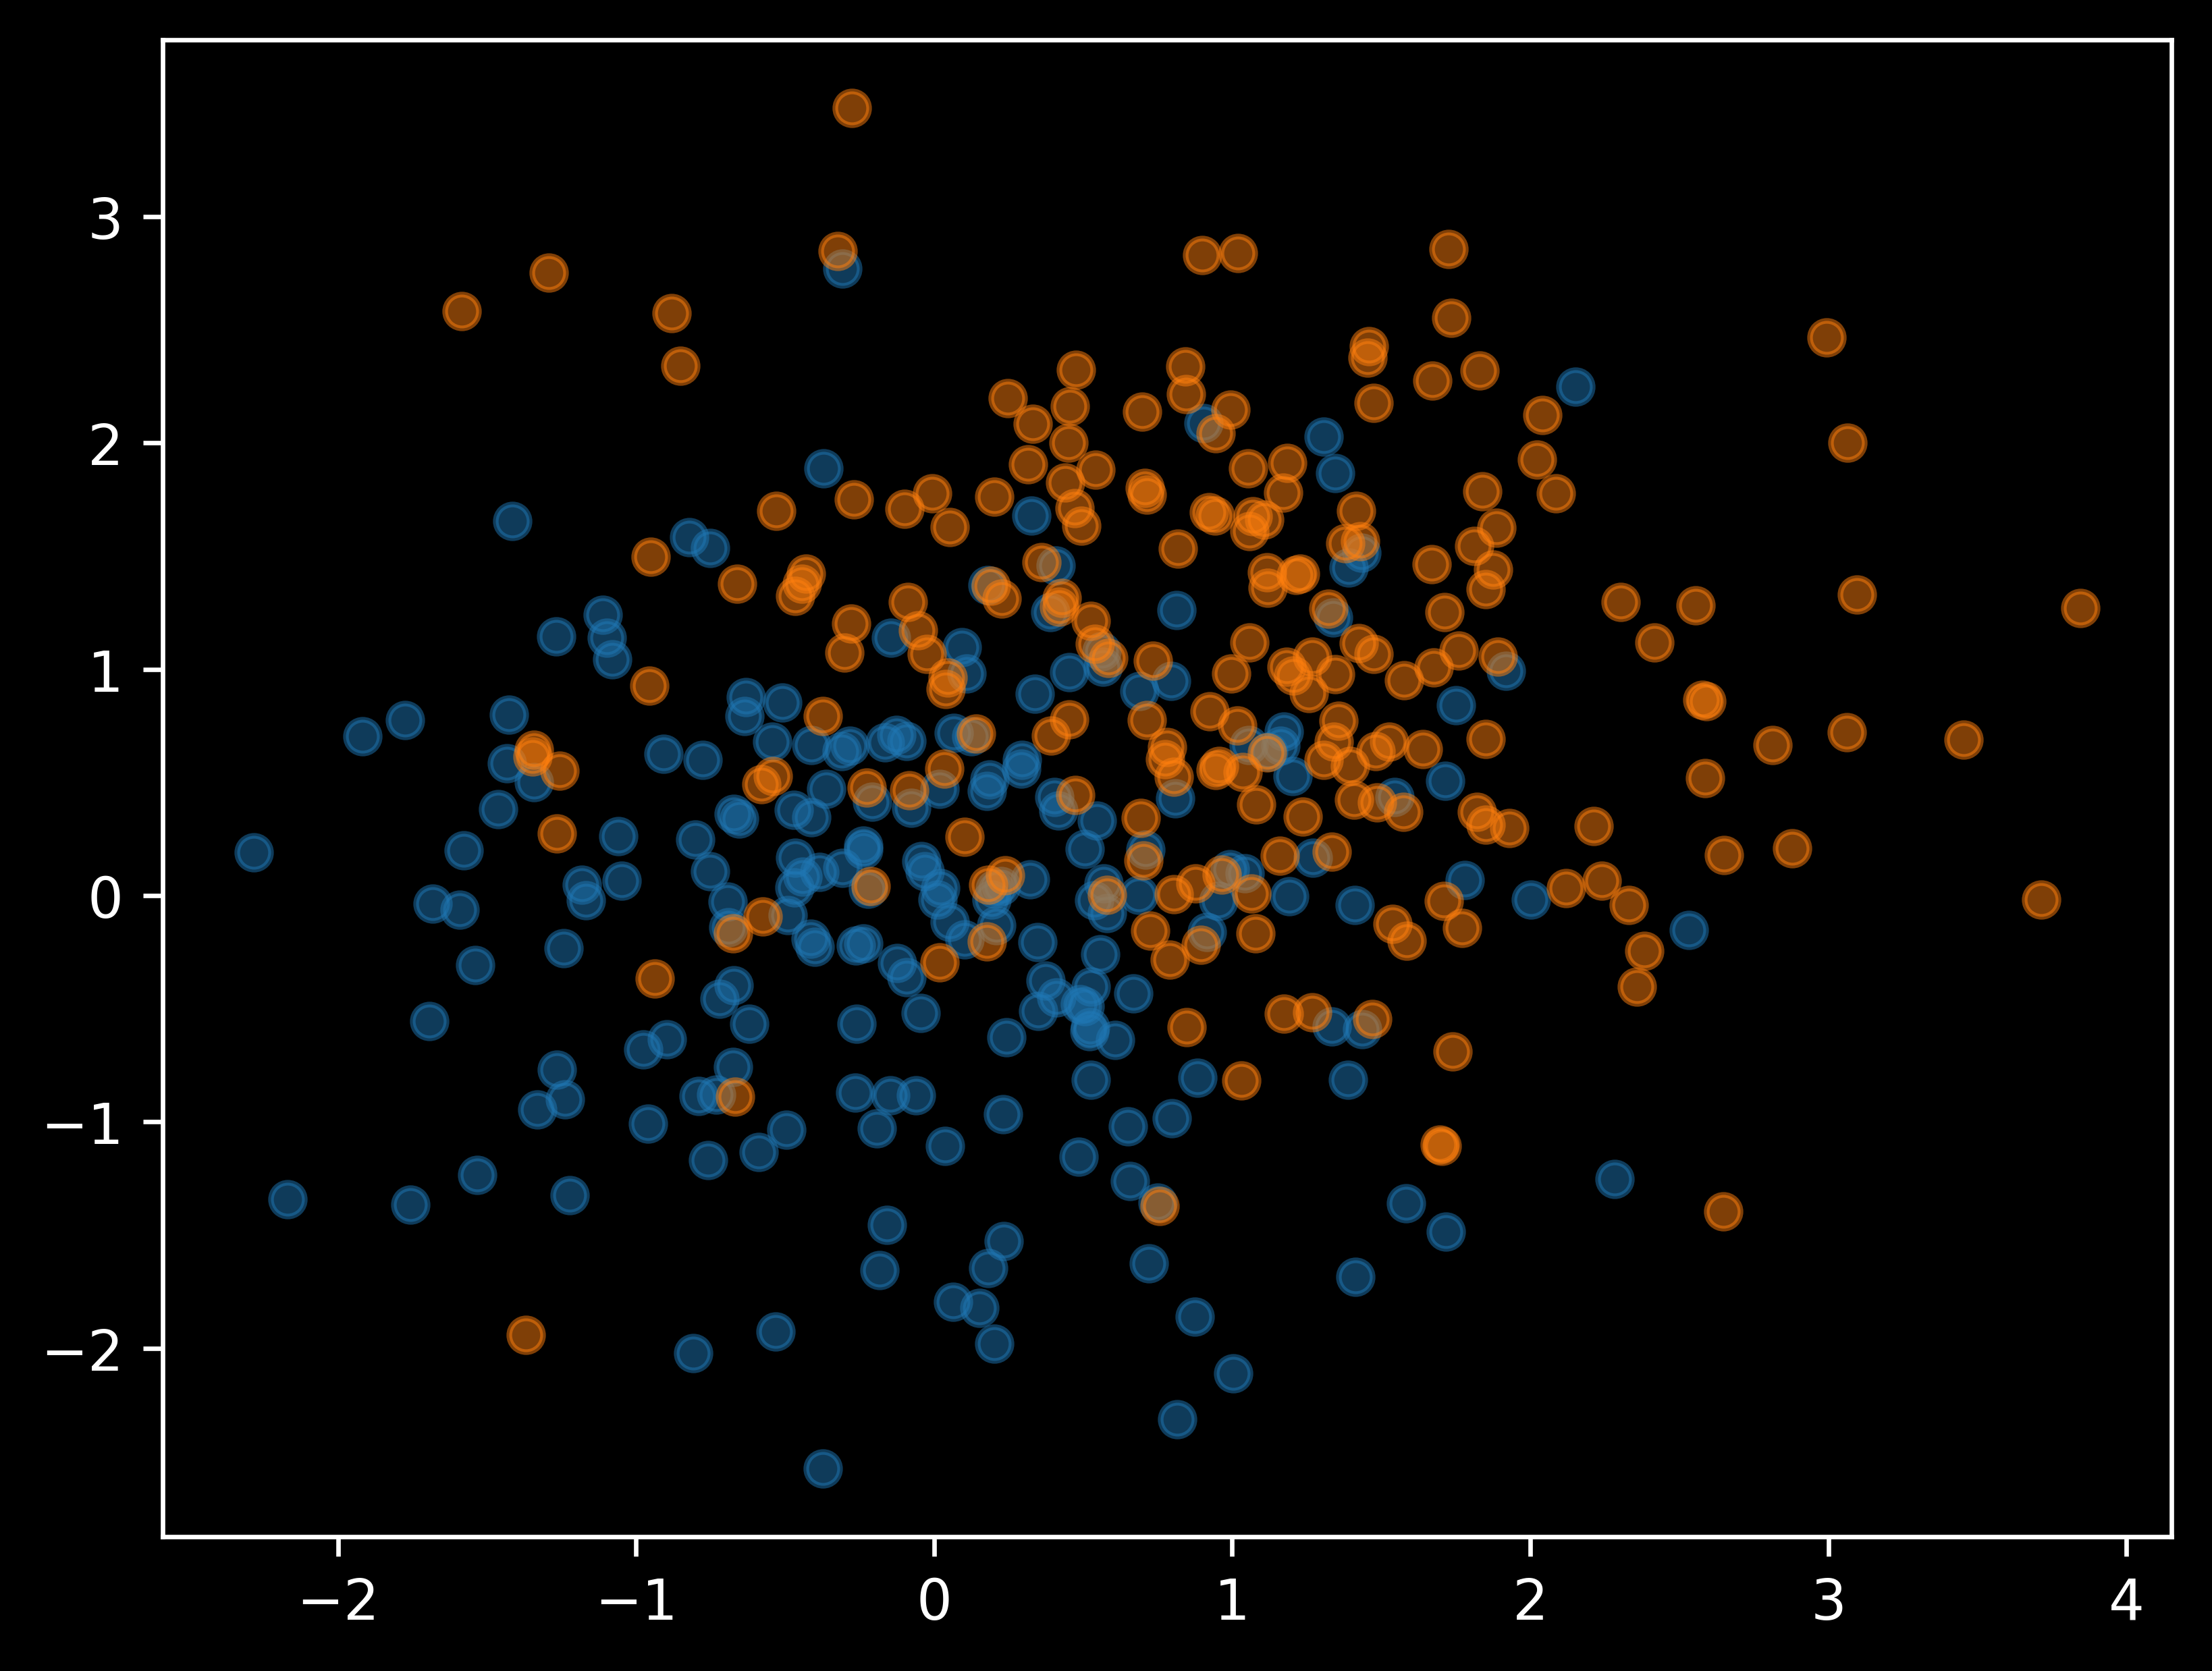
\includegraphics[width=\textwidth]{scatter_plot_multi}
  \end{minipage}
  \vfill
\end{frame}





\begin{frame}
  \vfill
  \centering
  \textbf{Tracer des histogrammes}
  \vfill
\end{frame}


{
  \setbeamercolor{background canvas}{bg=white}
  \frame{
    \vfill
    \centering
    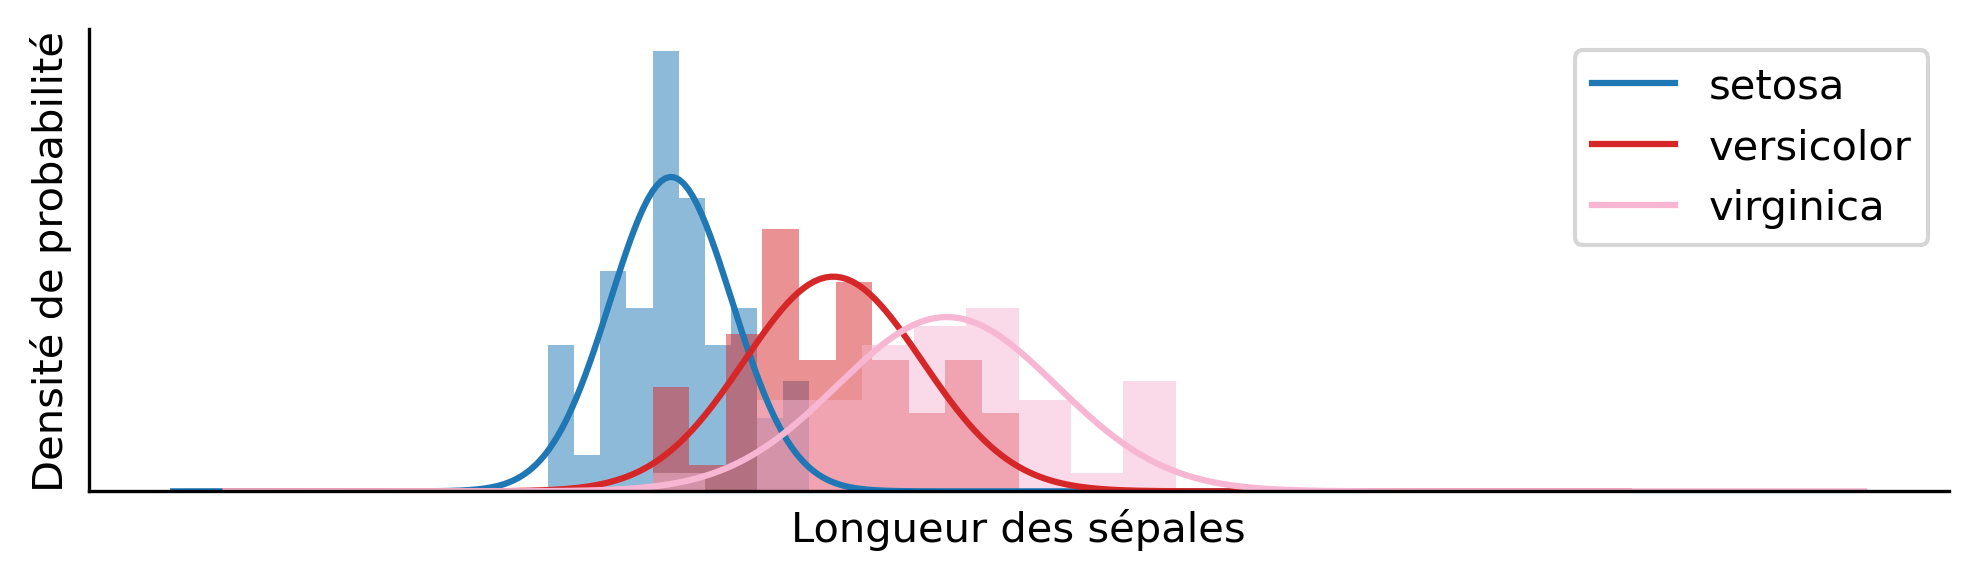
\includegraphics[width=\textwidth]{iris_dataset_bis}
    \vfill
  }
}

\begin{frame}[fragile]{}{}
  \vfill
  \begin{minipage}{.48\textwidth}
    \begin{lstlisting}[language=Python]
      # Donnees synthetiques.
      x = npr.randn(1000)

      # Cree la figure.
      plt.figure()

      # Plot l'histogramme.
      plt.hist(x)

      plt.show()
    \end{lstlisting}
  \end{minipage}%
  \hfill
  \begin{minipage}{.48\textwidth}
    \centering
    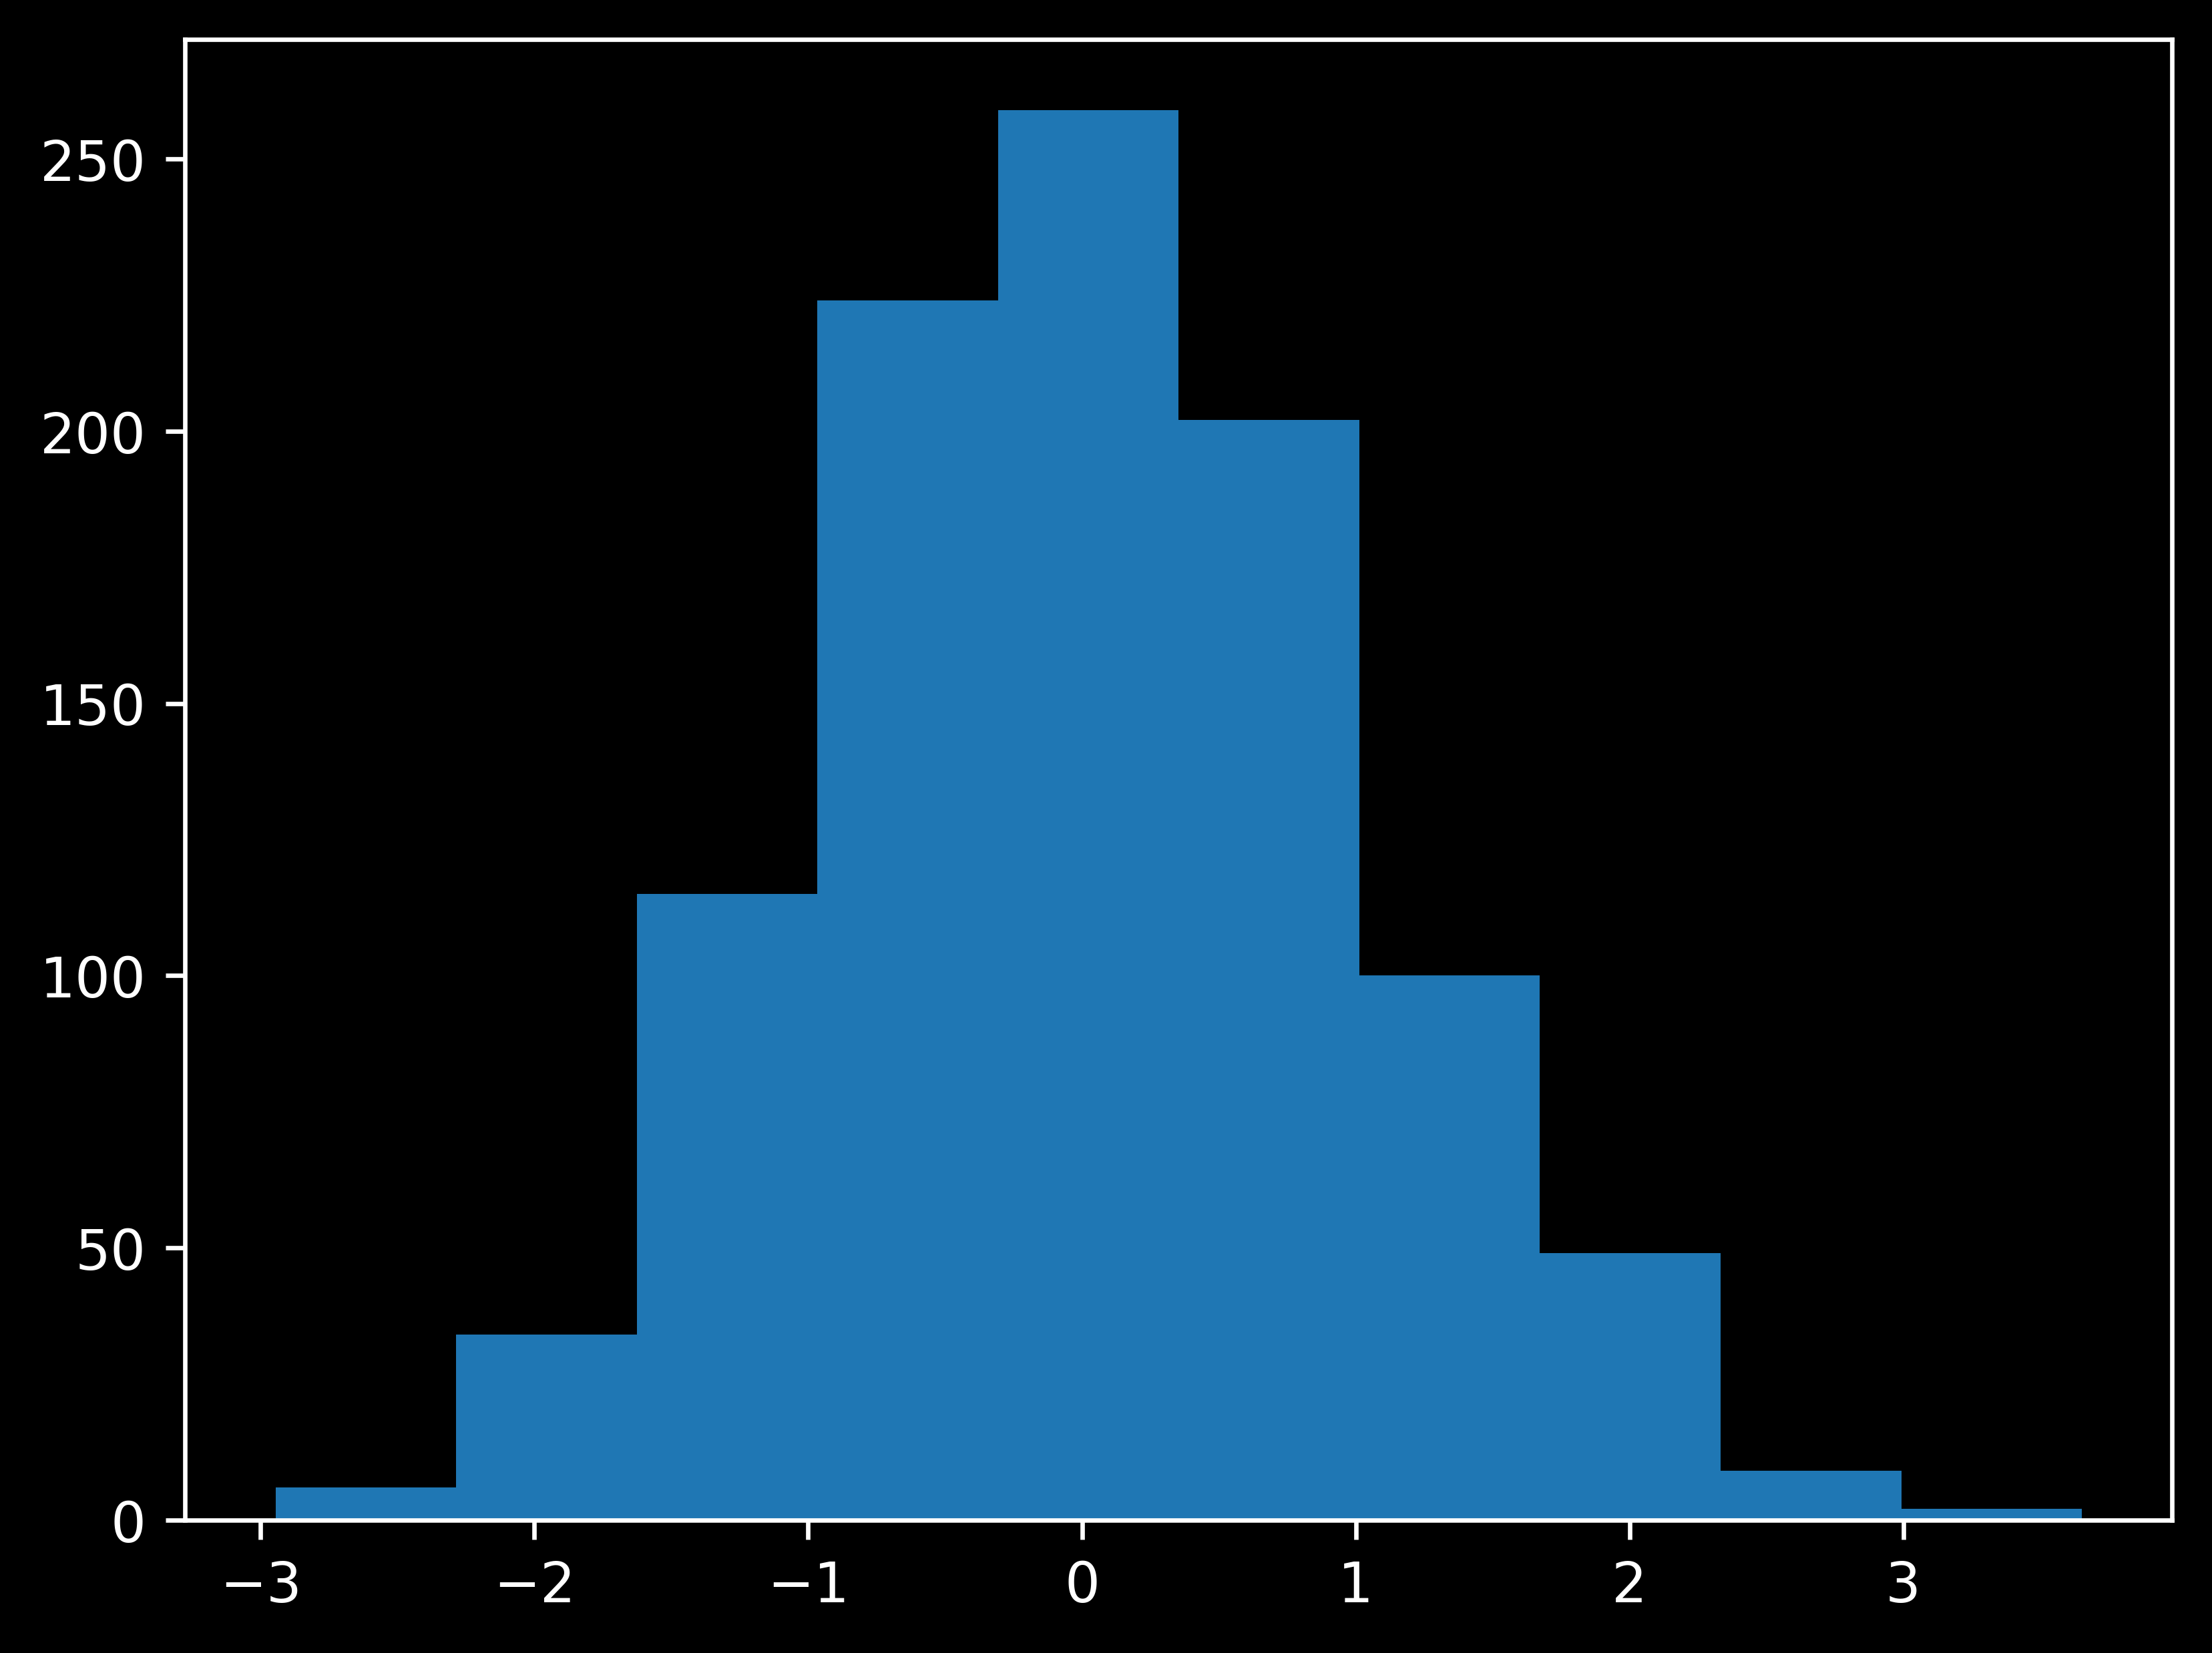
\includegraphics[width=\textwidth]{hist_plot_default}
  \end{minipage}
  \vfill
\end{frame}

\begin{frame}[fragile]{}{}
  \vfill
  \begin{minipage}{.48\textwidth}
    \begin{lstlisting}[language=Python]
      # Donnees synthetiques.
      x = npr.randn(1000)
      y = np.randn(100) + 1

      # Cree la figure.
      plt.figure()

      # Plot l'histogramme.
      plt.hist(x)
      plt.hist(y)

      plt.show()
    \end{lstlisting}
  \end{minipage}%
  \hfill
  \begin{minipage}{.48\textwidth}
    \centering
    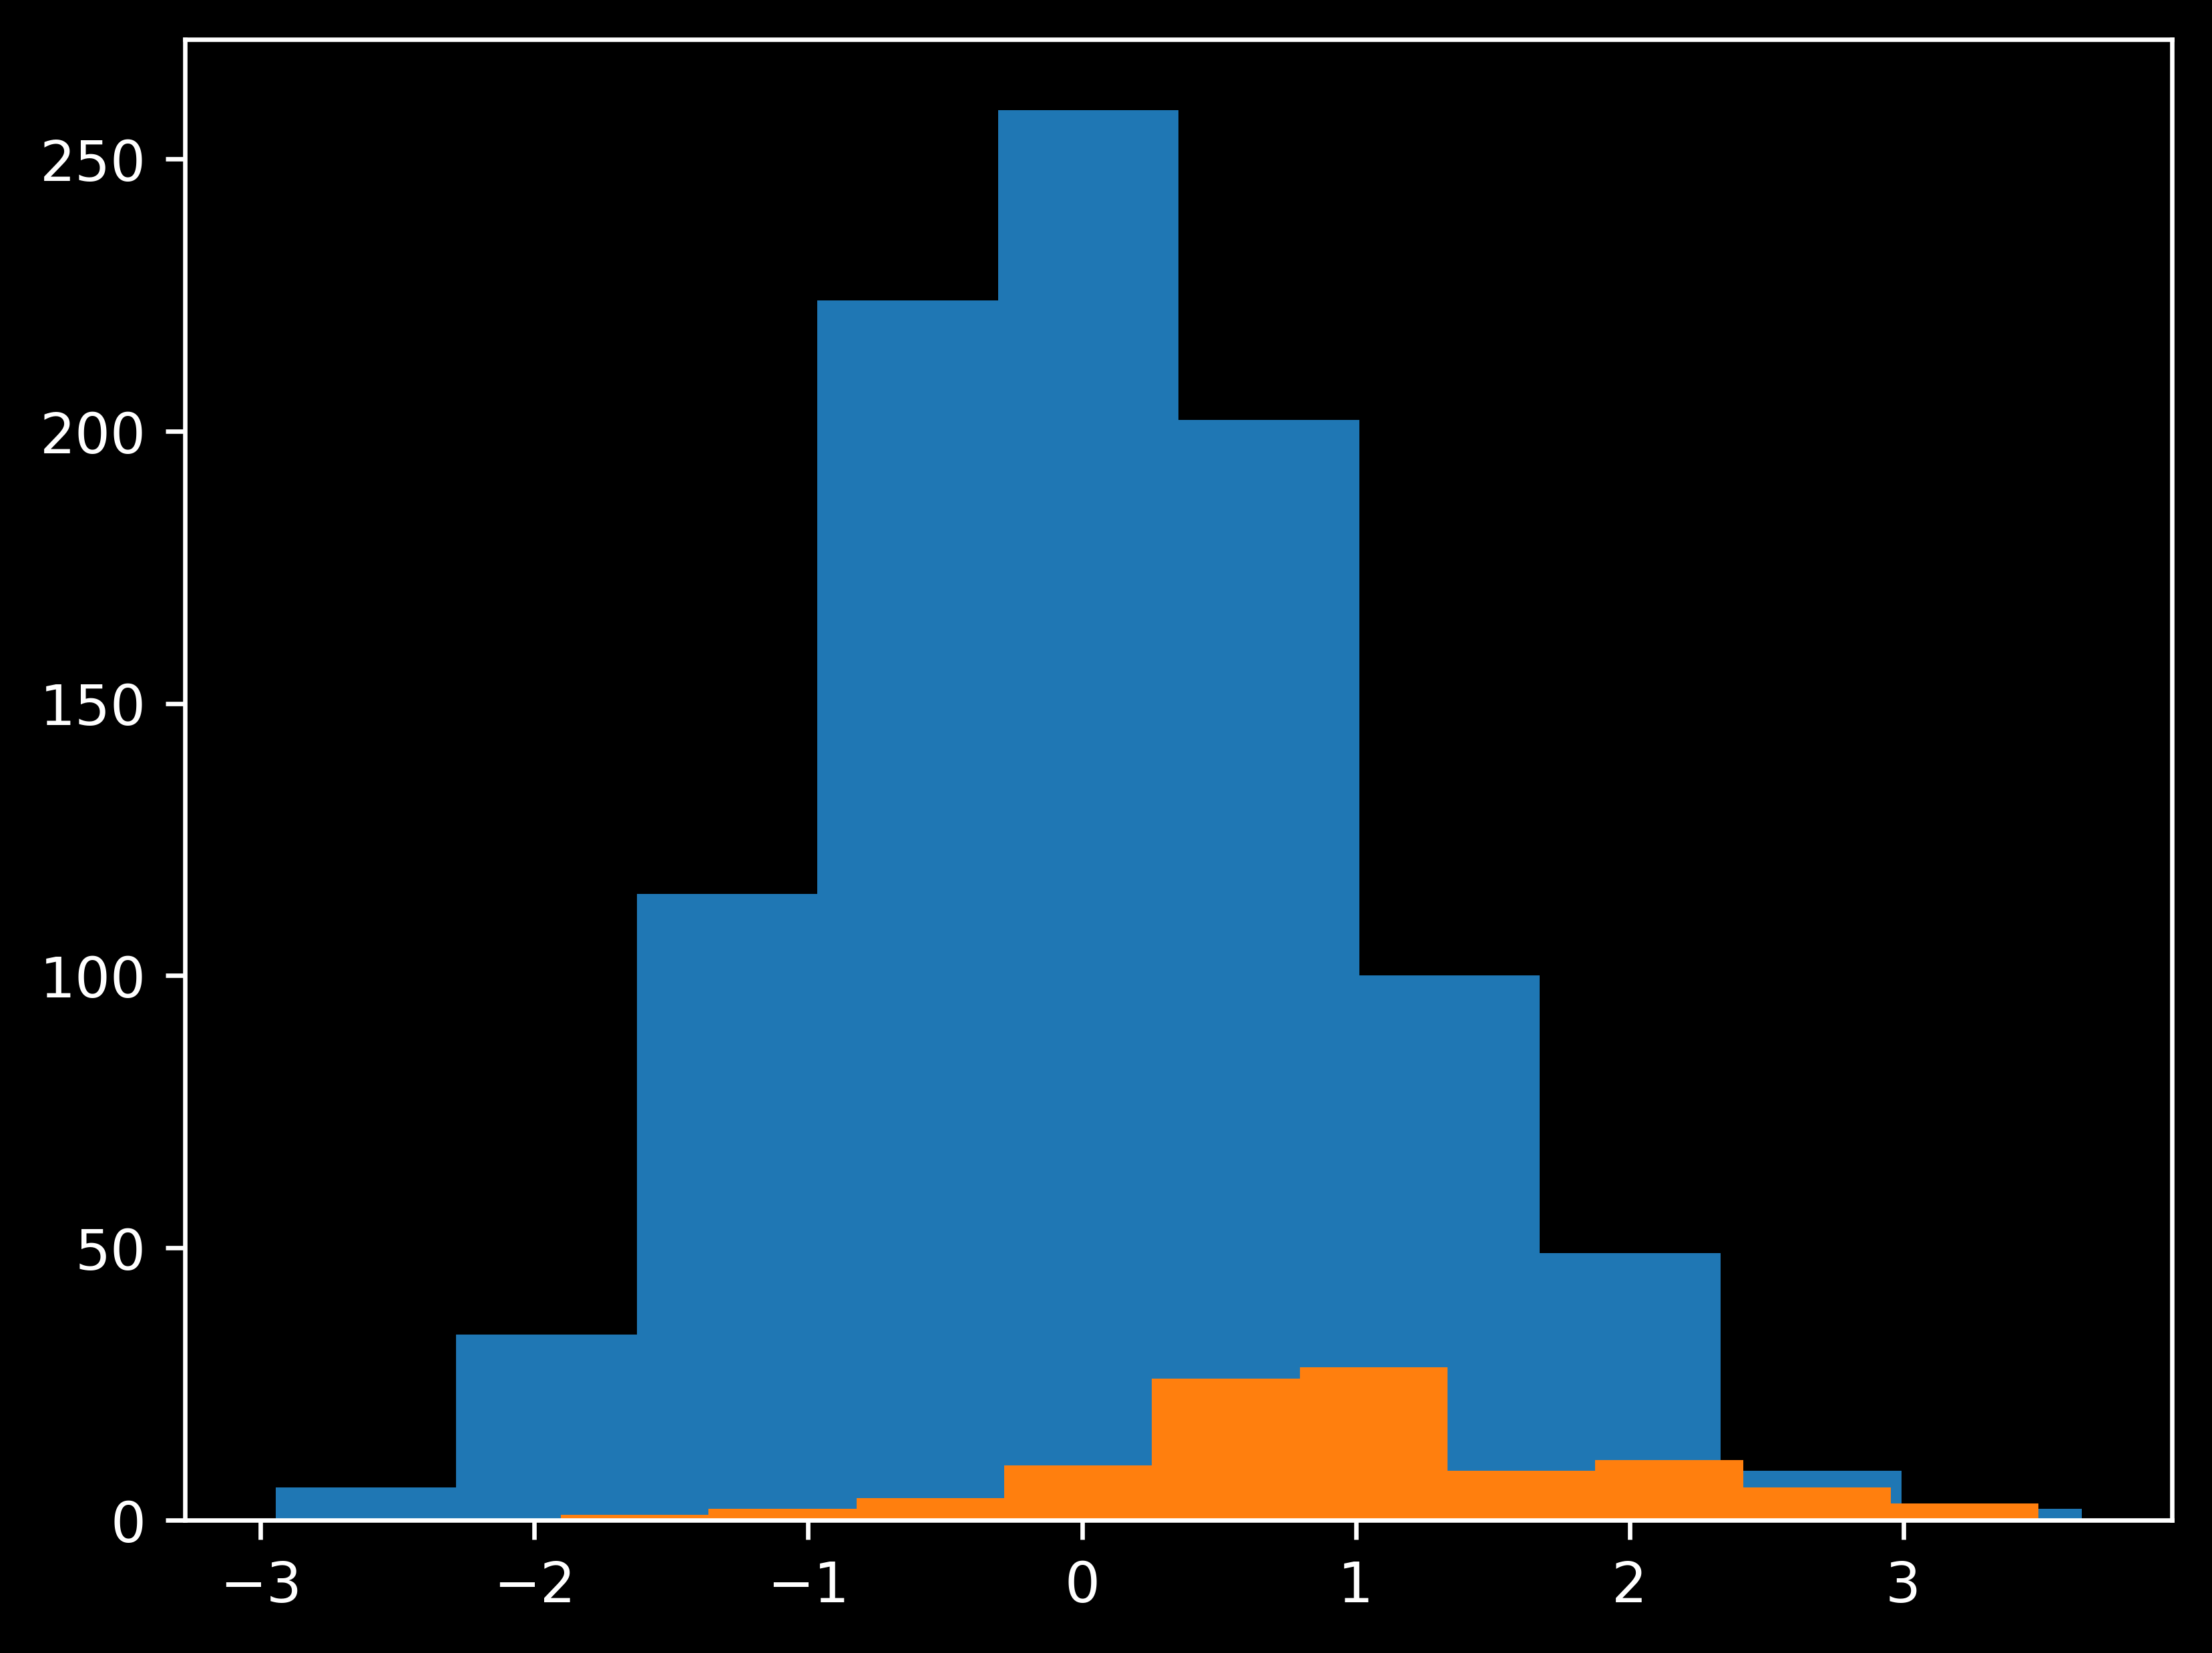
\includegraphics[width=\textwidth]{hist_plot_multi}
  \end{minipage}
  \vfill
\end{frame}


\begin{frame}[fragile]{}{}
  \vfill
  \begin{minipage}{.48\textwidth}
    \begin{lstlisting}[language=Python]
      # Normalisation.
      plt.hist(
          x,
          alpha=0.5,
          density=True)

      plt.hist(
          y,
          alpha=0.5,
          density=True)
    \end{lstlisting}
  \end{minipage}%
  \hfill
  \begin{minipage}{.48\textwidth}
    \centering
    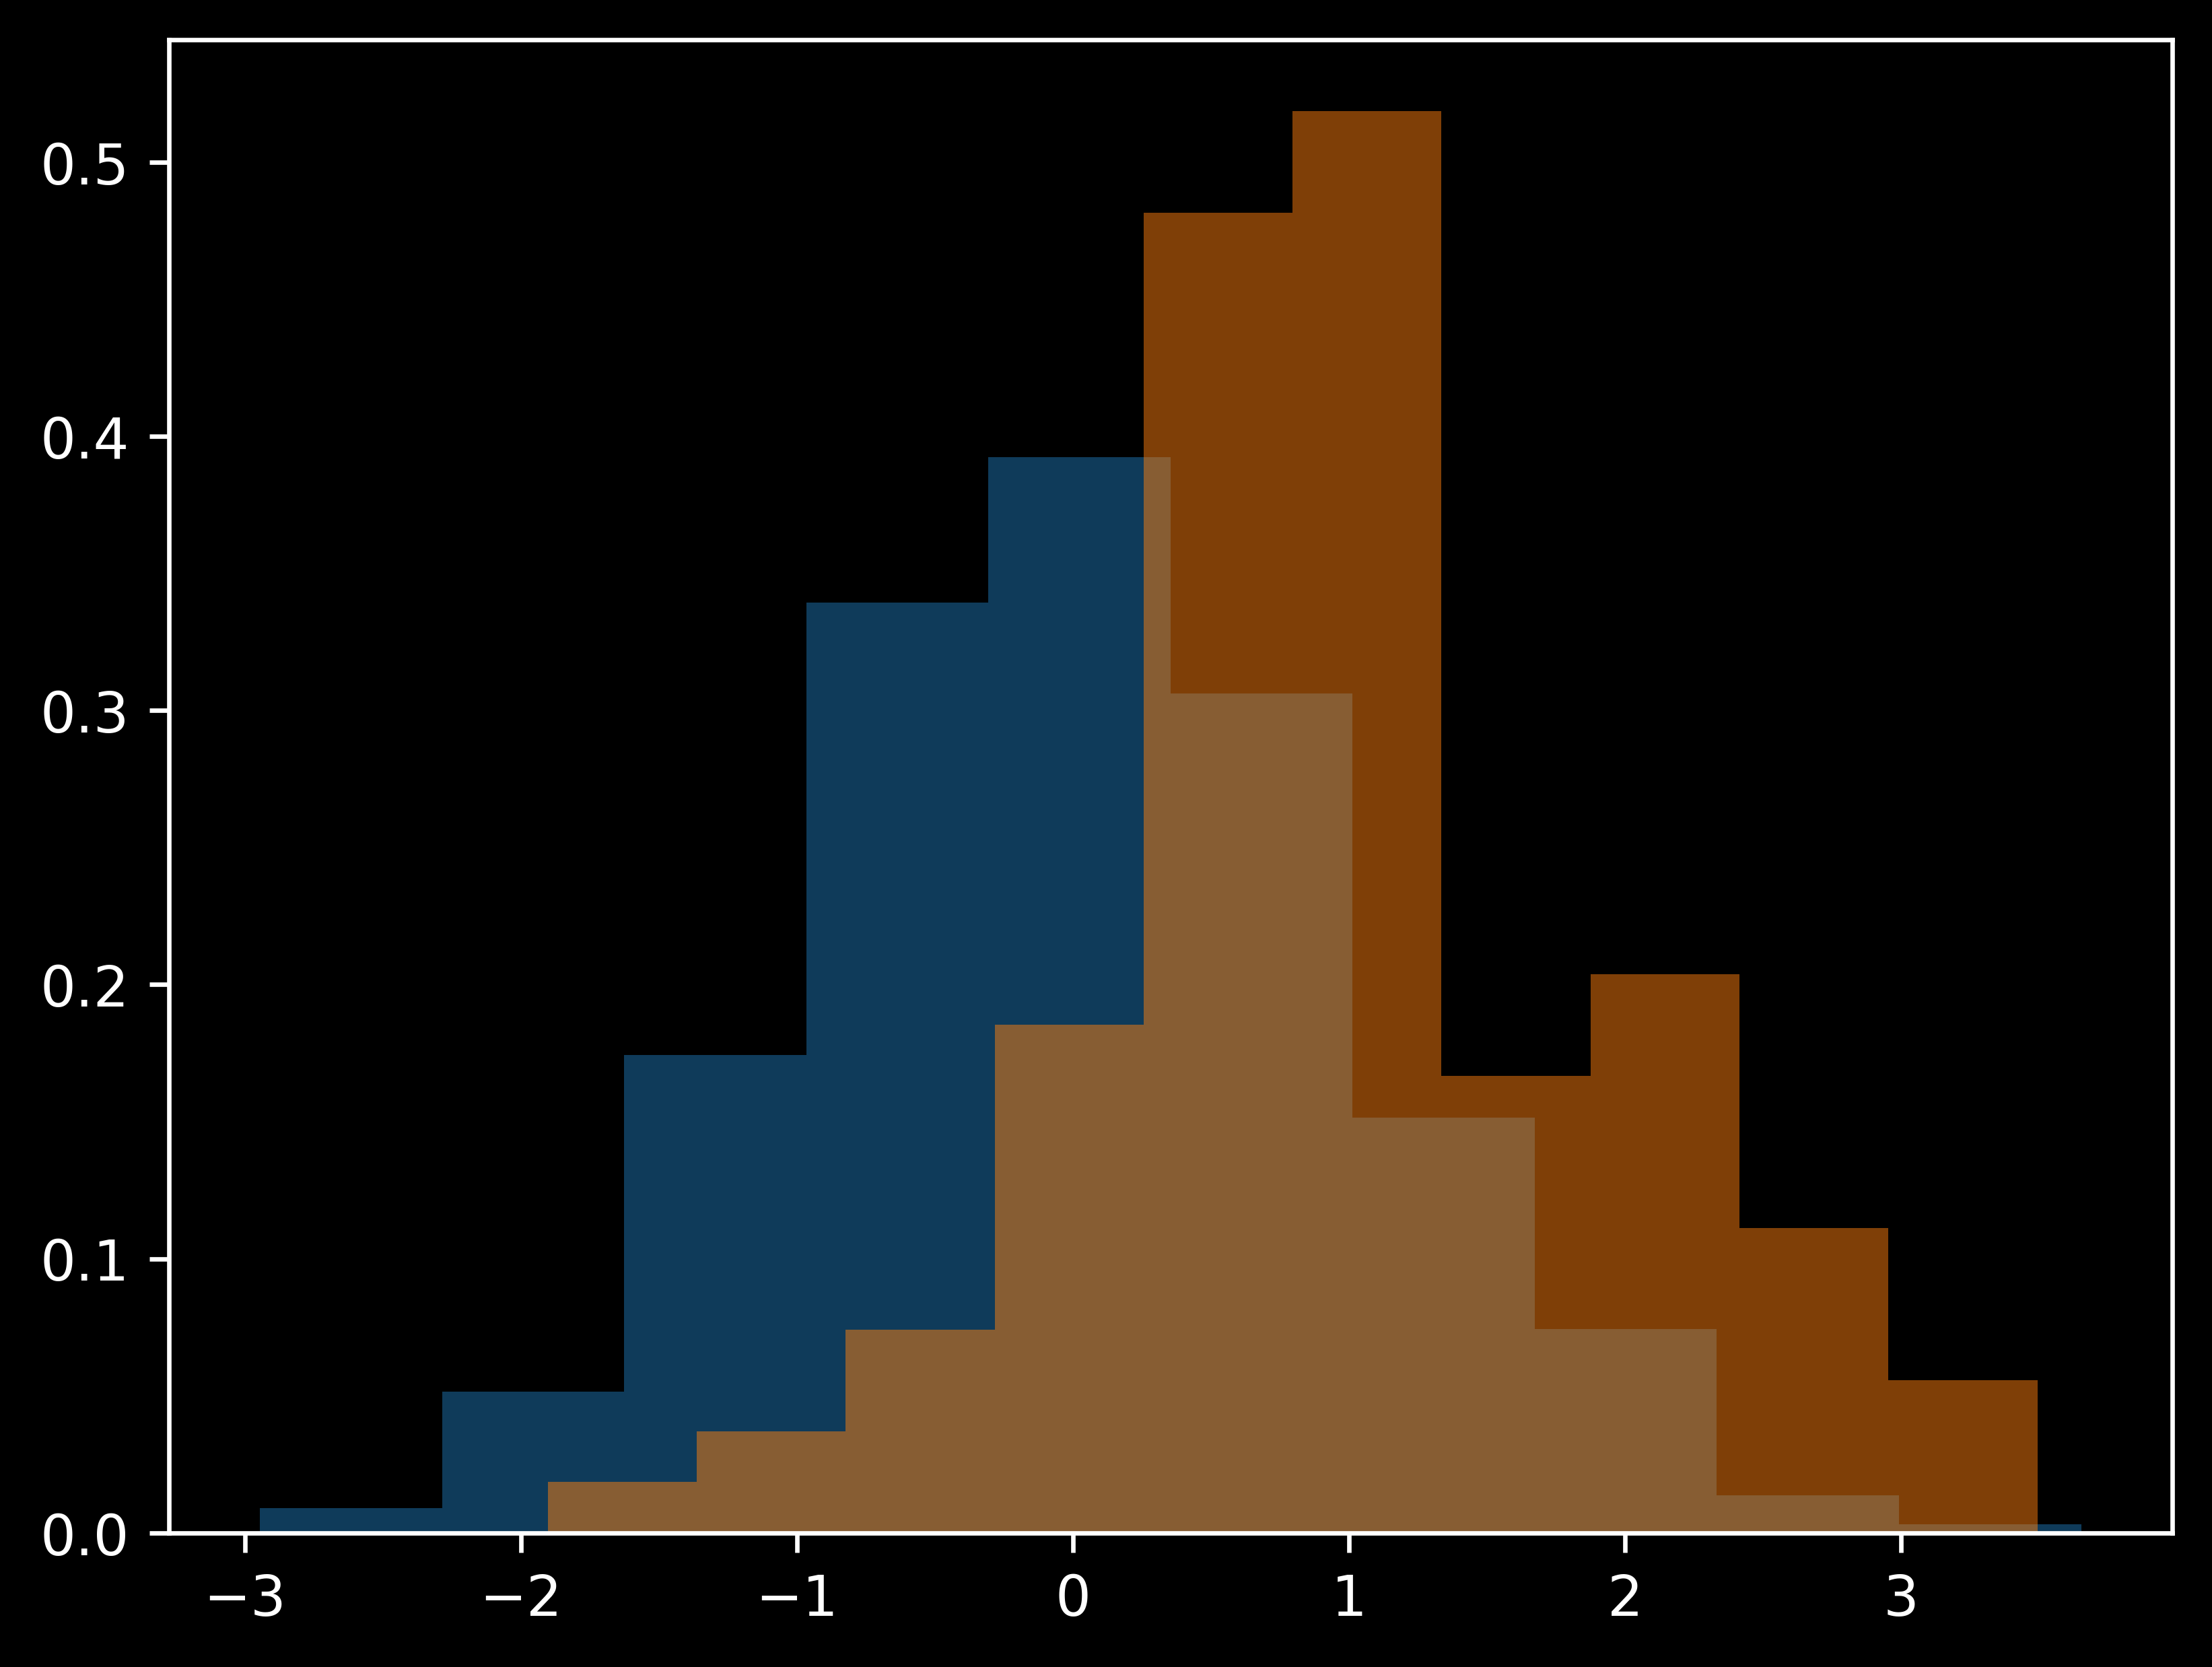
\includegraphics[width=\textwidth]{hist_plot_density}
  \end{minipage}
  \vfill
\end{frame}


\begin{frame}
  \centering

  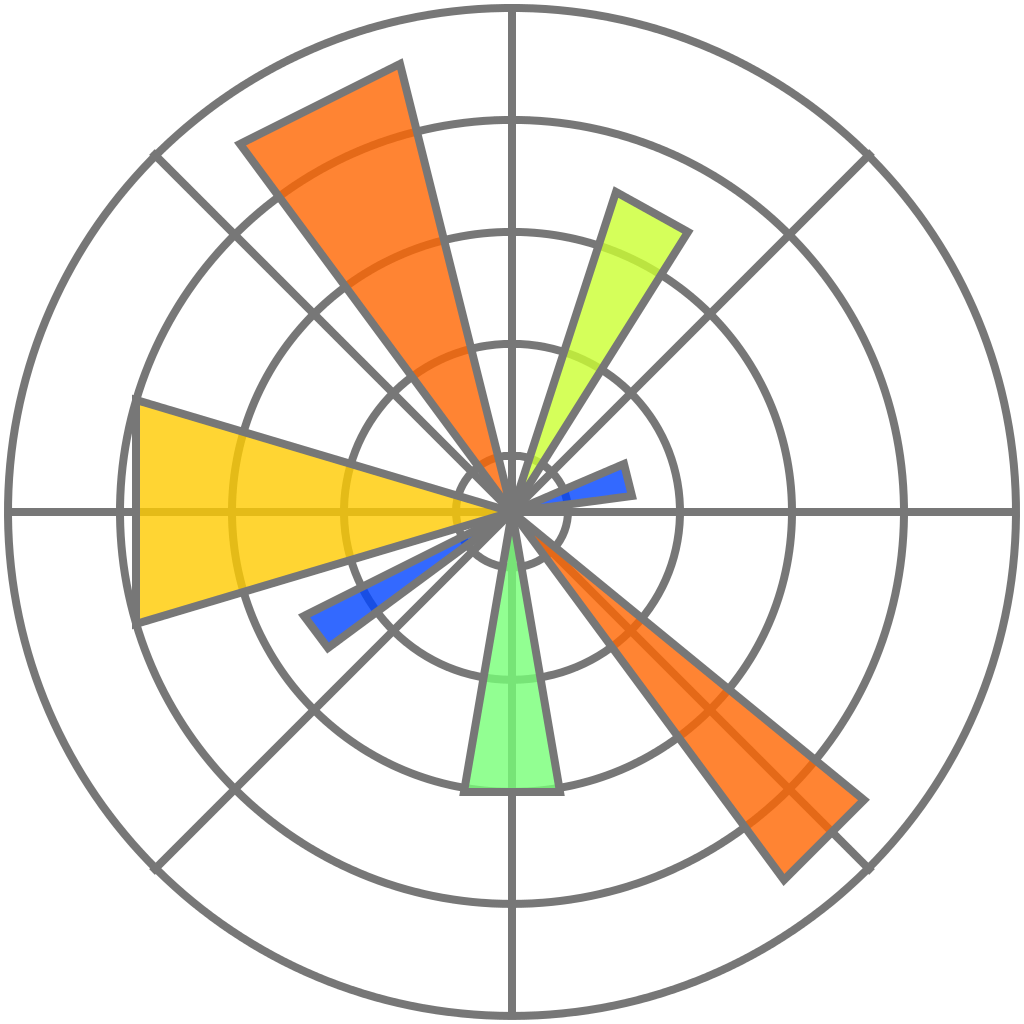
\includegraphics[width=.15\textwidth]{matplotlib_logo}

  Pour en savoir plus, rendez-vous sur \url{https://matplotlib.org/}
\end{frame}

\end{document}
